\documentclass[pdftex,final]{pittetd}
%final, makes pittetd's warnings (about things that might go against the Format Guidelines) into error messages. 
%Option 'sectionletters' numbers the chapters with Roman numerals (I, II, etc.), sections with 
%letters (A, B), subsections with numbers (1, 2), and subsubsections with lowercase letters (a, b). 
%The four levels of the enumerate environment receive the same treatment. Within the
%text, however, cross references (\ref} produce `the whole thing,' something like I.A.1 
%instead of only 1.

% Packages included in PittETD Template
% auto use this package and check for patches
\usewithpatch{graphicx} 
% manually use these packages
\usepackage{amsmath}
% manually check for patches
\patch{amsmath}
%\patch{amsthm}

% Jenna's commonly used packages
\usepackage{amssymb}
\usepackage{amsmath}
%\usepackage{amsthm}
\usepackage{graphics} % for improved inclusion of graphics
%\usepackage{wrapfig} % to include figure with text wrapping around it
%\usepackage{subcaption}
%\usepackage[margin=10pt,font=small,labelfont=bf]{caption}
\usepackage{algorithm}
%\usepackage{algorithmic}
\usepackage{algpseudocode}

% Bibliography
\bibliographystyle{apalike}

\title[Global Volume Registration for Motion Correction in rs-fMRIs]{Global Volume Registration for Multiple Motion Types in Resting-State Functional Magnetic Resonance Images}
% The optional argument is the 
% version of the title that will appear in Acrobat Reader's Document Info dialog box.
\author{Jenna Marie Schabdach}
\degree{B. S. Electrical Engineering, Drexel University, 2016\\M. S. Electrical Engineering, Drexel University, 2016\\M. S. Biomedical Informatics, University of Pittsburgh, 2018}

%\date{July 20th 1967}%             This date is the date of the thesis defense. Default is \today
% pittetd will use the current year unless otherwise indicated. So this command is not necessary.
\keywords{\LaTeX, pittetd, theses, format}% This list appears in the field 'Keywords' of Acrobat Reader's Document Info
%                                   dialog box, and also, optionally, after the abstract.
\subject{Schabdach Biomedical Informatics Dissertation}%              This fills in the 'Subject' field in Acrobat Reader's Document Info dialog box.
\school{Department of Biomedical Informatics}%    The name of the school will be preceeded by 'the' unless otherwise specified, as in:
%\school[certain]{department}

\begin{document}

\year{2019}  
%\chapterfloats%                    Un-comment this to get figures and tables numbered within chapters.
\maketitle
%
% For the committee membership page, you have to provide the names and affiliations of the members. The first one will 
% be treated by pittetd as the committee chair (thesis/dissertation advisor).
\committeemember{Dr. Ashok Panigrahy, Department of Biomedical Informatics}
%\coadvisor{Second advisor, Dept. Aff.}%         This is used if there are two advisors.
\committeemember{Dr. Douglas Landsittal, Department of Biomedical Informatics}
\committeemember{Dr. Jenna Gaessar, Dept.\ Aff.}
\committeemember{Dr. Shaym Visweswaran, Department of Biomedical Informatics}
% etc., as many as needed. For master's theses, the committee may be omitted, naming only the advisor.
\school{School of Medicine}
\makecommittee
%\copyrightpage                     Uncomment this to get a copyright page.
\begin{abstract}
INSERT ABSTRACT HERE
\end{abstract}
% If you say \begin{abstract}[Keywords:] instead of the simple \begin{abstract}, a list of the keywords is appended.
% The list comes from the \keywords command above.
% The starred version \begin{abstract*} typesets the word `ABSTRACT' on the top of the page
\tableofcontents
%\listoftables                      Pittetd will complain if you tell it to create a list of tables when there are no
%                                   tables (as in this sample file). Uncomment this command if you have tables.
%\listoffigures                     Obvious analogous for figures.
%\preface
% This is the text of the preface, with acknowledgments, dedication, etc. It is optional, and you create, as shown, by 
% just saying \preface and starting the preface's actual text. Note that 'foreword' is no longer acceptable as title
% for this preliminary.
%
%Conventions, such as notation (nomenclature) and abbreviations, don't receive their own preliminary page. They can be included as an appendix, or as part of the introduction.


% Add in chapters here
\chapter{Introduction}

Resting-state functional magnetic resonance imaging (rs-fMRI) measures the blood oxygen level dependent signal in an organ or organ system. This property makes rs-fMRI an invaluable tool for evaluating a patient's neurodevelopmental status or examining functional networks in his brain. To gather enough data to fully evaluate these networks, a series of image volumes must be acquired over a period of several minutes. In a standard rs-fMRI (?), one new image volume is obtained approximately once every two to three seconds. To gather high quality data on such a short timescale, the rs-fMRI suffers from two major limitations: rs-fMR images have low physical resolution and are highly susceptible to motion. The first limitation can be addressed by obtaining an MR image with high physical resolution and registering the rs-fMRI to this structural image, but the second limitation requires the patient to remain as still as possible for the entire duration of the scan. This task is particularly difficult for populations of certain ages or populations who suffer from conditions that affect neurodevelopment. As a result, it is common for an image from a member of one of these populations to contain too much motion to be used in clinical or research applications.

Various behavioral and XX protocols have been developed in an attempt to prevent patients from moving during MRI scans, though many of these protocols are not applicable to younger populations. In particular, a neonate or fetus cannot understand instructions to stay still, and young children who can understand the command have difficulty following it. Sedation is not advisable for these young populations. After a rs-fMR image is acquired, however, it is possible to reduce the positional effects of motion in the image sequence.

Limitations of traditional methods

DAG-based registration

Apply DAG-based registration to neonates and preadolesents

Real goal is to develop a method of registering fetal brain and placental images so that we can further examine the relationship between placental oxygen levels and fetal brain development. Longitudinally, this technique can be used to determine how placental oxygen flow and fetal brain development impact a patient over the course of his or her life. Once the relationship between the placenta and fetal brain development is better understood, we can determine a set of neuroprotective interventions to employ for at-risk patients before they are born.
\chapter{Background}
The topics treated in this chapter can be somewhat obscure. For humanitarian considerations, the chapter will be subdivided.

\section{RESTING-STATE NETWORKS}

The idea of a neuronal network which operated when a person is at rest was proposed in 2001, and then confirmed in 2003 \cite{Raichle2001} \cite{Greicius2003}. Resting-state networks are recorded using resting-state functional magnetic resonance images (rs-fMRIs). rs-fMRIs are sequences of image volumes acquired over a period of a few minutes while the patient is in a task-free state. The image volumes themselves have relatively low spatial resolution when compared to structural MRIs, but their temporal resolution is significantly higher as a new volume is acquired every two to three seconds. Each volume records the blood oxygen level dependent (BOLD) signals within the brain at that point in time. 

The BOLD signals in rs-fMRI image sequences are analyzed using a process called functional connectivity analysis. Functional connectivity analysis identifies patterns and networks of brain activity. Because the patient is not performing a specific task during a rs-fMRI acquisition, these resting-state networks have the potential to reveal valuable information about a patient's neurodevelopmental status. Some functional connectivity analysis studies have lead to the discoveries of links between specific disruptions in these naturally occurring networks and neurodevelopmental diseases such as autism and attention deficit hyperactivity disorder \cite{Assaf2010} \cite{Zang2007}. With further refinements of both acquisition techniques and characterization of these functional networks, clinicians may be able to use rs-fMRI in early detection protocols to evaluate the neurodevelopmental status of infants and neonates, and in personalized care by identifying patients who may benefit from certain therapies or neuroprotective interventions.

\section{MEASURING THE EFFECTS OF MOTION}

Due to their low spatial and high temporal resolutions, rs-fMRIs are highly susceptible to motion. Even the smallest movement can alter the position of the patient enough to cause the voxels to record signals from different brain regions and tissue types. Even if the movement does not significantly change the recorded position of the subject, it impacts the established spin gradients, which introduces artifacts into the image sequence. Movements cause the orientation of existing spin gradients to change, and the gradients require time to realign to the magnetic field. This recovery time often results in a decrease in the global signal in frames obtained over the following 8-10 seconds, which can affect the functional connectivity analysis \cite{Power2014}.

The effects of motion on rs-fMRIs can be clearly divided into two categories: the effect on patient position and the effect on the recorded BOLD signal.

The effect of motion on patient position is measured in terms of the difference in position between temporally neighboring image volumes. The difference in position is determined using metrics calculated by performing rigid volume registration on the two volumes. 
In rigid volume registration, one volume is chosen as the reference volume and the other is considered the moving volume. The reference volume remains stationary while the moving volume is translated and rotated in three-dimensional space on top of it. The registration is considered successfully complete when the position of the patient in the moving volume matches the position in the reference volume. The three translation and three rotation parameters used to achieve this alignment are used to calculate the positional change between the image volumes, which is often called the framewise displacement (FD). 

Several researchers have proposed different methods for calculating the FD. Power et al., Jenkinson et al., and Dosenbach et al. each propose a slightly different method for calculating the FD \cite{Power2012} \cite{Jenkinson2002} \cite{Dosenbach2017}. All three FD calculations produce correlated metrics: the FD metric proposed by Power et al. produces measurements approximately twice as large as the metric proposed by Jenkinson et al., and Dosenbach et al. reported a high correlation between their FD and Power’s FD \cite{Yan2013a} \cite{Dosenbach2017}.

Signal change 
Even the smallest movement can impact the recorded BOLD signal for the following eight to ten seconds [CITE].


An rs-fMRI must (contain only low amounts of motion) for functional connectivity analysis to be successful. There is some debate a

\section{MOTION PREVENTION}

Sedation can be used for some medical image acquisitions, but it is not appropriate for all patient populations or imaging modalities. 

\section{MOTION CORRECTION}

\section{VOLUME REGISTRATION}

Liao et al. suggested that a rs-fMRI sequence could be viewed as a hidden Markov model, and reflected this idea in their suggested registration framework \cite{Liao2016}. Their framework uses the transformation of the previous volume to the reference volume as the initial transformation for the current volume and the reference volume. 



%\section{MAGNETIC RESONANCE IMAGING}
%
%Magnetic resonance imaging is a technique used in medicine to obtain in vivo images of different organ systems. The patient is placed in a static magnetic field and electromagnetic pulses are used to briefly induce a secondary magnetic field.
%
%One type of MRI is resting state functional MRI (rs-fMRI). rs-fMRI is 
%
%
%\section{THE CHALLENGE OF MOTION}%            Remember to capitalize the sections (otherwise, the bookmark will be lowercase)
%
%Patient movement is a challenge across all modalities of medical imaging, but rs-fMRI is particularly sensitive to it. Various preventative, 
%
%An rs-fMRI is considered usable if it contains at least 5 minutes of low motion data.
%
%\subsection{•}
%
%
%
%\subsection{First subsection of the section}
%This is well-known topic, and we shall discuss it no more.
%\subsection{Second subsection of the section}
%This is a very complicated topic and we shall discuss it in our next paper.\textsl{•}

\chapter{DATA}
\label{ch5:data}

The data used to test the hypothesis and aims introduced in the previous chapter are drawn from four clinical groups and  a set of simulated rs-fMRI sequences. In this chapter, we will first discuss the clinical images, which were taken from several prospective studies of congenital heart defects in pediatric patients as well as a prospective study of Alzheimer's disease in an aging population. Subjects from these studies were chosen because patient motion causes problems in MR images for the entire patient lifespan, though patients may exhibit different types of motion at different stages of life. 

Then we will discuss how we overcame the lack of objective ground truth in medical imaging research by developing a mechanism to simulate brain activity, scanner noise, and motion in rs-fMRI sequences.

\section{Clinical Cohorts}

The phrases congenital heart defects (CHDs) and congenital heart disease (CHD) both refer to defects in the heart or the vessels around the heart. CHDs affect how blood moves into, through, and away from the heart. 
CHD has a worldwide prevalence of about 8 per 1000 live births, meaning about 1.35 million children are born with CHD every year. %Since the survivability of CHD has increased from 10\% to 90\%, the medical community is faced with a growing, aging population of CHD patients. 

In this section, we provide a general overview of the impact of CHD on a global scale, the process for diagnosis, and additional risks associated with CHD. We then discuss the process of diagnosing neurodevelopmental comorbidities occurring with CHD and the impact of improved medical care on the CHD population. We end this section with a description of the four populations from which we obtained clinical rs-fMRI sequences.


\subsection{CHD Background}

\begin{figure}
\centering
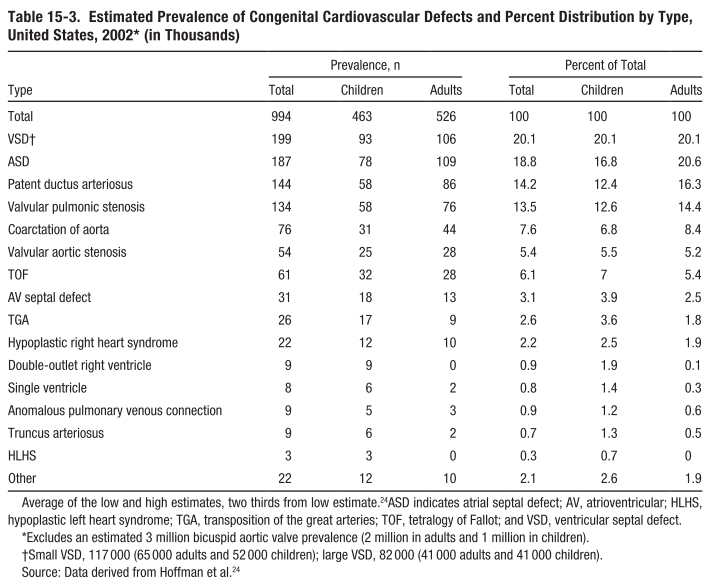
\includegraphics[width=0.6\textwidth]{5/chd-defects-usa.png}
\caption{Table of prevalences of congenital heart defects borrowed temporarily from \cite{Mozaffarian2016}.}
\label{ch5:fig:usa-defects-prev}
\end{figure}

CHD consists of a variety of defects which can affect any combination of the vessels and chambers of the heart with varying degrees of severity. The defects prevent the cardiopulmonary system as a whole from functioning correctly, but pinpointing and treating the defects effectively can be a complex process. It is important to note that each defect type has a different prevalence, a different treatment plan, and different expected outcomes. A breakdown of prevalence rates of some of the most common lesion types can be seen in Figure \ref{ch5:fig:usa-defects-prev}. % See (16)

% Causes of CHD: genetic syndromes, single gene mutations, environmental exposure, and unknown
Different presentations of CHD are associated with a number of different genetic and environmental factors \cite{Mozaffarian2016}. Genetic conditions such as Down syndrome, Turner syndrome, 22q11 deletion syndrome, Williams syndrome, and Noonan syndrome are associated with certain CHD presentations. Maternal behaviors such as smoking and binge drinking are known to cause heart problems in the fetus. Other maternal risk factors are obesity, folate deficiency, and living at a high altitude. Paternal exposure to phthalates, anesthesia, sympathomimetic medications, pesticides, and solvents may increase the risk of the fetus for developing CHD. While there are quite a few factors in this list, there are many CHD cases whose causes are unknown.

Once a patient is diagnosed with one of these defects or a cause of the CHD is identified, the specific nature of his case must be clearly documented. The documentation of CHD using the International Classification of Diseases, Ninth Revision, Clinical Modification (ICD-9-CM) has 25 high level codes representing various presentations of CHD, but these codes used alone are often not sufficient for describing a patient's true condition \cite{Mozaffarian2016}. Additional ICD-9-CM codes should be used to communicate the finer details of a patient's condition, if they are available. %something about how ICD codes make it easier to

The incidence of CHD in live births vary across countries and continents. The United States reports approximately 4-10 CHD case per 1000 live births. Europe and Asia see about 6.9 and 9.3 CHD cases per 1000 live births, though smaller studies have been conducted in many countries to measure local prevalence \cite{Mozaffarian2016}. In China, the incidence of CHD ranges from 8.98 to 11.1 per 1000 live births \cite{Zhao2019} \cite{Qu2016}. 
A pair of studies from Iran report incidences of 8.6 and 12.3 per 1000 live births, though the studies note that they were performed in different geographical locations with different populations within the country \cite{Nikyar2011} \cite{Rahim2008}.
One report from Dharan reports an incidence of 5.8 per 1000 patients admitted to a tertiary care hospital over a 12 month period \cite{Shah2008}. A study of newborns at one hospital in New Delhi, India claims an incidence of 3.9 per 1000 live births, though this rate may be a poor estimate as there is a significant delay between patient birth and referral to a cardiac center in India \cite{Khalil1994} \cite{Saxena2005}.

These incidence rates should be analyzed with some caution. In many cases, the reported rates were based on medical records. Medical records are not always correct; it is well known that human error can lead to a medical record lacking information or containing incorrect information. The only way for a person to have a medical record is for him or her to go to a medical center. Not everyone who has CHD is able to seek medical help, often because of their geographical locations or their income. Even if a patient is able to seek medical help, the availability of proper cardiac care varies between and within countries. However, it is generally expected that CHD incidence rates will increase as screening tools and treatments become more effective and more widespread, leading to earlier detection of defects.
 
% Diagnosis
Currently, the process of detecting and diagnosing CHD can begin before birth. A specialized ultrasound test called fetal echocardiography can detect heart abnormalities as early as the second trimester of the pregnancy. People who learn they are pregnant with a fetus who shows signs of CHD may choose to handle this information by opting for termination or pursuing a more detailed diagnosis. Additional tests, such as amniocentesis and follow-up ultrasounds may be used to determine treatment options before the patient is born. Generally, severe CHD cases present and are detected at earlier stages of life, but minor defects may not become apparent until the patient is older. Tests used to diagnose CHD in postnatal patients include electro- and echo-cardiograms, chest x-rays, pulse oximetry, exercise stress tests, computed tomography or MRI scans, and cardiac catheterization. Treatment of different defects varies from monitoring and medication to surgery and cardiac implants.

\begin{figure}
\centering
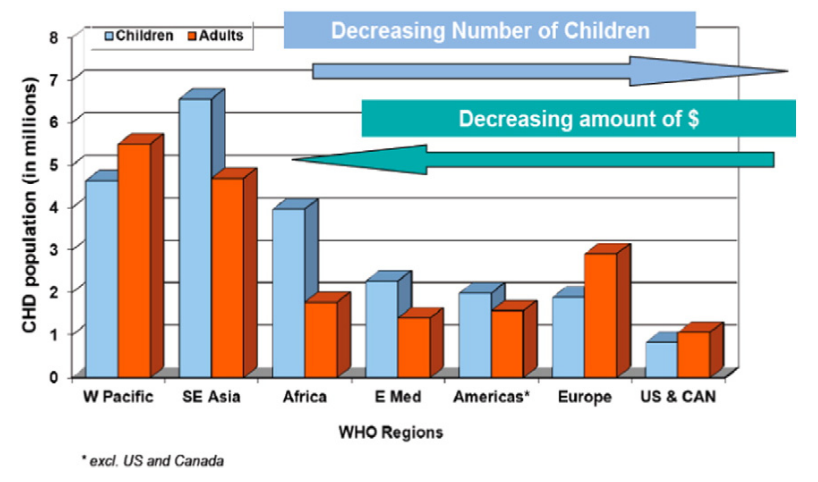
\includegraphics[width=0.7\textwidth]{5/CHD-burden-webb.png}
\caption{Estimated CHD burden in World Health Organization (WHO) regions using incidence rates of approximately 12/1000 and 4/1000 in children and adults, respectively \cite{Webb2015}.}
\label{ch5:fig:CHD-burden}
\end{figure}

%Depending on the cause of the 
The cost of diagnostic techniques and treatment plans impose different levels of financial burden on CHD patients and their families. Certain defects require complex, expensive surgical repairs while others can be treated with less expensive approaches \cite{Mozaffarian2016}. The burden of CHD across the globe was outlined by Webb et al \cite{Webb2015}. Their figure illustrating the prevalence of CHD and the availability of funds with which to treat it can be see in Figure \ref{ch5:fig:CHD-burden}. As the overall mortality of CHD declines, the burden of CHD is expected to increase \cite{Mozaffarian2016}.

% Complications and risks
Unfortunately, the cost of treating CHD is not the only burden a patient must undergo. Patients with CHD are also at increased risk for heart failure and infections \cite{Mozaffarian2016}. Children with CHD are at 19-fold risk for stroke compared to their healthy counterparts \cite{Fox2015}. In a study of Swedish citizens born between 1970 and 1993, Giang et al compared the prevalence of cardiac conditions in patients with and without CHD \cite{Giang2018}. They found that patients who had a CHD diagnosis were at about eight times higher risk for intracerebral hemorrhage and subarachnoid hemorrhage than their non-CHD counterparts. The CHD patients were also more likely to suffer from arrhythmia and heart failure. 

% When are patients diagnosed?
% Expected lifespan
% Treatment plan
% Financial burden

However, cardiac conditions are not the only complications CHD must deal with. Many of these patients also suffer from neurocognitive disorders that co-occur with CHD. Early research in this area focuses on the neurodevelopmental status of neonatal patients pre- and post-surgical intervention. One theory was that some factor or factors in the surgical intervention caused brain injuries in the patients. This idea proved to be inaccurate when researchers began detecting neurological malformations \textit{in utero}.

In a systematic review of available literature regarding prenatal and postnatal presurgical CHD cases and neurodevelopmental outcomes, Mebius et al. identify two theories about the causality of  neurodevelopmental delays and CHD \cite{Mebius2017}. The first theory is that abnormalities in the cardiac system prevent the developing brain from receiving enough oxygen and nutrients, which disrupts prenatal brain development. The second theory is that faulty genetic pathways used during both cardiac and brain development cause both conditions to co-occur. However, 11 articles Mebius et al. found during their review that are related to bloodflow through the umbilical artery suggest a third theory. During the prenatal period, a fetus receives oxygen from the mother via the placenta. If the placenta was not functioning correctly, it could lead to the fetus receiving not enough oxygen. Lower quantities of oxygen throughout prenatal development could potentially cause problems both in brain and cardiac growth. The 11 articles have contradictory results, but some researchers are currently investigating the role of the placenta in CHD and prenatal brain development.

Survival of CHD patients to adulthood has increased from 10\% to 90\% over the last several decades as CHD diagnostic tools and treatments have improved.  Currently, Webb et al. estimate that at least 12 to 34 million adults have CHD, and this number is expected to increase \cite{Webb2015}. The impact of the combination of CHD and neurological conditions throughout a patient's lifetime is starting to be explored. The aging of the CHD population has also sparked interest in the relationships between CHD and adult-stage neurological disorders such as dementia and Alzheimer's. 

While the purpose of this study is not to focus on CHD patients, we chose to use CHD and aging brain images in support of research being performed in the area of relationships between CHD and neurodevelopment.

%To address:
%\begin{itemize}
%\item Common combinations
%\item Joint treatment?
%\item Additional risks?
%\item Joint financial and emotional burden on caretakers? 
%\item CHD, neuro, and aging? Dementia/Alzheimer's? Recent data ... MIND neuroimaging ancillary r01 dec 17
%\end{itemize}


\subsection{Identifying Neurocognitive Disorders}

Neurocognitive disorders are usually diagnosed using at least one of many psychological survey-based evaluations, but these methods are subjective. rs-fMRIs could be used to identify patients who have functional connectivity patterns associated with different neurocognitive disorders, and eventually may be used to identify patients who are at risk for developing these disorders.

\subsubsection{Patient Surveys}

Surveys known to be used for studying the relationship between CHD and neurodevelopment are

\begin{itemize}
\item National Institute of Health Toolbox (3 - 85 years): ``Performance tests of cognitive, motor, and sensory function and self-reported measures of emotional function for adults and children in the general population and those living with a chronic condition''.

\item Sue Beers (4 - 18 years [not inclusive of 18 years]): WASI-II, NEPSY-2, WRAML-2, D-KEFS, WISC-IV, Grooved Pegboard, BRIEF, Beery-Buktenica VMI, ASRS, Conners-3, BASC-II, ABAS-II, PedsQL General, PedsQL Cardiac, Pictoral Scale Self Perception Profile.

\item SVR-III NDT (9 - 13 years [not inclusive of 13 years]): WIAT, NEPSY, WRAML, D-KEFS, WISC-V, Grooved Pegboard, BRIEF, Beery-Buktenica VMI, ASRS, Conners ADHD Index, BASC-II, ABAS-3, PedsQL General, PedsQL Cardiac

\item Bayley Scales of Infant and Toddler Development -III (1 - 24 months): Subtests include cognitive, language, social-emotional, motor, and adaptive behavior tests \cite{Mebius2017}.

\item Battelle Developmental Inventory (Birth - 8 years [not inclusive of 8 years]): Subsets include cognition, communication, social-emotional development, physical development, and adaptive behavior.

\item Developmental Assessment of Young Children (Birth - 6 years [not inclusive of 6 years]): Subtests include cognition, communication, social-emotional development, physical development, and adaptive behavior.

\item Preschool Language Scale + Receptive-Expressive Emergent Language (Birth - 3 years): Total language, auditory comprehension, expressive communication, articulation, receptive language, expressive language, and inventory of vocabulary words.

\item Peabody Developmental Motor Scales (Birth - 5 years): Subtests include reflexes, stationary, locomotion, object manipulation, grasping, visual-motor integration
\end{itemize}

The goal of these surveys is to compare the patient's cognitive function and neurological functions to expected milestones. Certain deviations from certain milestones are indicative of different disorders.

\subsection{Study Cohorts}

The rs-fMRIs used in this study were gathered as part of ongoing studies of the relationship between CHD and neurodevelopment. Data from the CHD/neurodevelopment studies was obtained through studies approved by the IRB at the Children's Hospital of Pittsburgh of UPMC and the University of Pittsburgh. All data is stored and accessed in compliance with HIPPA policies.

The subjects included in this analysis fall into three age groups: neonatal, preadolescent, and fetal. To summarize the cohorts, there were 163 brain rs-fMRIs obtained for the neonatal cohort, 546 brain rs-fMRIs obtained for the preadolescent cohort, and 124 brain rs-fMRIs obtained for the fetal cohort. The fetal cohort also contains 106 rs-fMRIs of the placenta. The race, ethnicity, and gender counts for these three cohorts can be seen in Figures  In the following sections, we describe each cohort in detail. 

\begin{figure}
\centering
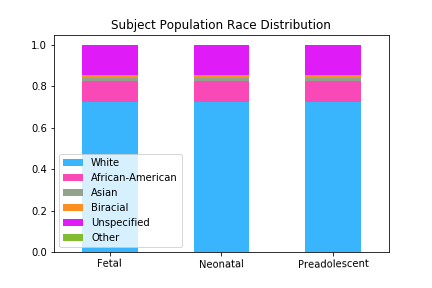
\includegraphics[width=.75\textwidth]{5/demo_clinical_subj_race.png}
\caption{Distribution of subject races for all three cohorts.}
\label{ch5:clinical:race}
\end{figure}%
%
\begin{figure}
\centering
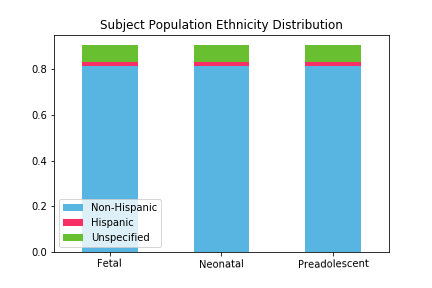
\includegraphics[width=.75\textwidth]{5/demo_clinical_subj_ethnicity.png}
\caption{Distribution of subject ethnicities for all three cohorts.}
\label{ch5:clinical:eth}
\end{figure}

\begin{figure}
\centering
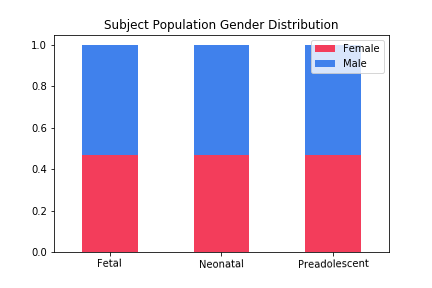
\includegraphics[width=.75\textwidth]{5/demo_clinical_subj_gender.png}
\caption{Distribution of subject genders for all three cohorts.}
\label{ch5:clinical:gender}
\end{figure}

\subsubsection{Neonatal Cohort and Images}

Neonatal subjects have been recruited as part of a prospective observational study. This cohort was scanned at two sites. At Site 1, the subjects were scanned using either a 3T Skyra (Siemans AG, Erlangen, Germany) or a 3T GE . At Site 2, the subjects were scanned using a 3T Philips (*).

The subjects were unsedated during the scans and a ``feed and bundle'' protocol was used to prevent motion during the scans \cite{Windram2011}. The newborns were positioned in the coil to minimize head tilting. Newborns were fitted with earplugs (Quiet Earplugs; Sperian Hearing Protection, San Diego, CA) and neonatal ear muffs (MiniMuffs; Natus, San Carlos, CA). An MR-compatible vital signs monitoring system (Veris, MEDRAD, Inc. Indianola, PA) was used to monitor neonatal vital signs. All scans were performed using a multi-channel head coil. The parameters for the resting-state BOLD MR scans were FOV=240 mm and TE/TR=32/2020 ms with interplane resolution of 4x4 mm, slice thickness of 4 mm, and 4 mm space between slices. The acquired images contained 150 volumes where each volume consisted of 64x64x32 voxels$^3$.

\begin{figure}
\centering
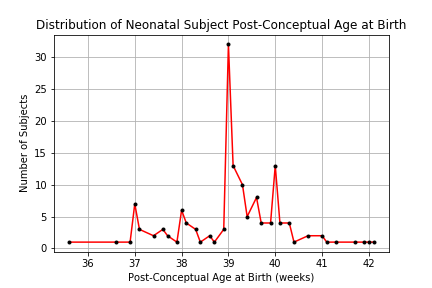
\includegraphics[width=.75\textwidth]{5/demo_neonate_subj_pca.png}
\caption{The distribution of post-conceptual ages at birth of all neonatal subjects.}
\label{ch5:neonates:birthpca}
\end{figure}

\begin{figure}
\centering
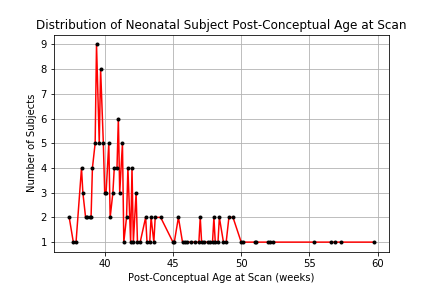
\includegraphics[width=.75\textwidth]{5/demo_neonate_scan_pca.png}
\caption{The distribution of post-conceptual ages at the time of the scan of all neonatal subjects.}
\label{ch5:neonates:scanpca}
\end{figure}

A total of 149 patients were recruited. The average post-conceptual age of the patients at birth was 39.08 weeks and they were on average 42.64 weeks post-conception at the time of the scan. The distribution of post-conceptual ages of the subjects at birth and at the time of the scan can be seen in Figure \ref{ch5:neonates:birthpca} and Figure \ref{ch5:neonates:scanpca}. 

\begin{figure}
\centering
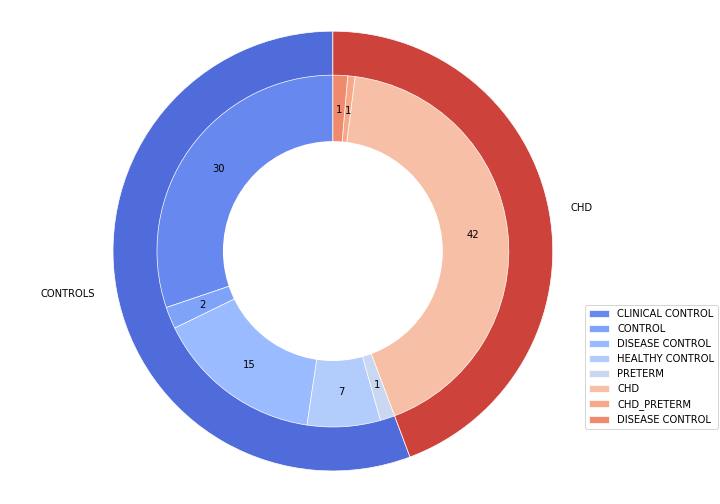
\includegraphics[width=1.0\textwidth]{5/demo_neonate_subj_cohort.png}
\caption{The breakdown of subject groups contained in the Control and CHD neonatal cohorts.}
\label{ch5:neonates:cohorts}
\end{figure}

The subjects were a mix of control subjects and CHD subjects. A comprehensive breakdown description of the subgroups within these two cohorts can be seen in Figure \ref{ch5:neonates:cohorts}. In this figure, the term ``Control'' encompasses both healthy full-term subjects, healthy pre-term subjects, and non-CHD clinical subjects (clinical control and disease control). The CHD group is composed of subjects diagnosed with CHD who were either born full-term or pre-term. Of the entire cohort, 14 subjects underwent two scanning sessions resulting in 163 rs-fMRI scans.

As the neonates were most often asleep during the scan, they exhibit less motion overall compared to our other clinical cohorts. The high-motion neonates are an obvious exception to this concept, but many of the high-motion images contained long periods where the subject was stationary. Applying both the DAG-based framework and the traditional registration framework to these images provided the opportunity to compare the performances of both registration frameworks to each other in the context of the usability gold standard thresholds. 

\subsubsection{Preadolescent Subject Population and Images}

As part of a multicenter study of CHD in preadolescents, we collected rs-fMRIs from nine sites throughout the United States. These images were of patients in the age range of 9 to 13 years who either had CHD or were healthy with no neurocognitive impairments. In addition to the MRI scans, subjects who participated in this study were asked to participate in additional testing  either to determine their neurocognitive outcome status or to perform genetic analyses. % (GET DETAILS FROM NANCY).

\textbf{Preadolescent Cohort.} The multicenter imaging study of preadolescent subjects provides a unique opportunity to evaluate the efficacy of the DAG-based framework on a large subject cohort containing variable amounts of motion. The outcome of this experiment will be used in the next experiment to determine if there are any site-specific or vendor-specific variables influencing patient motion.

%\begin{itemize}
%\item How were the images gathered?
%\item How were the patients recruited?
%\item What are the imaging protocol details?
%\item What other information was collected?
%\end{itemize}

\subsubsection{Fetal Subject Population and Images}

%Real goal is to develop a method of registering fetal brain and placental images so that we can further examine the relationship between placental oxygen levels and fetal brain development. Longitudinally, this technique can be used to determine how placental oxygen flow and fetal brain development impact a patient over the course of his or her life. Once the relationship between the placenta and fetal brain development is better understood, we can determine a set of neuroprotective interventions to employ for at-risk patients before they are born.

Fetal subjects have different constraints on their physical environment than neonates, preadolescents, and adults. As a result, they exhibit unique patterns of motion. The previous subject cohorts discussed in this chapter have the following commonalities: the subject experiences the full effects of gravity, the subject is lying on his back in an MRI scanner, and the subject's head motion is limited by the head coil within the MRI. Any motion in these images is a direct result of the subject himself moving, whether passively (cardiac motion and breathing) or actively (fidgeting or looking around).

A fetal subject is scanned in vivo. He is suspended in amniotic fluid within his mother. The amniotic fluid has buoyancy that reduces the effects of gravity and allows a fetal subject significant freedom of movement. The fetus can rotate, shift, and flip in ways that can only be accomplished when floating in a body of water. The properties of the uterus constrain the physical space in which a motion could occur, but not as much as the head coil and gravity do to the other patient cohorts. A fetus is not guaranteed to be in any specific position at the start of the scan: the scan begins when the mother is ready, not when the fetus achieves a certain pose. 

The fetal subjects underwent fetal echocardiography scans in a cardiac clinic to determine whether they were healthy or had a form of CHD. They were then scanned on an MRI scanner. Images of the fetal brain and the placenta were acquired for each subject. 

We are interested in both the fetal brain and placental images for our work because of the relationship between placenta and brain development. However, these organs have very different physical properties. The fetal brain is a rigid structure floating and moving within the amneotic fluid. It undergoes translation and rotation as a single unit due to passive and active maternal and fetal motions. The placenta, on the other hand, is anchored in place on the uterine wall. It may undergo small translations or rotations due to maternal motion, but it will respond differently to fetal motion. Fetal motions cause nonlinear deformations of the pliable placenta that can only be adequately accounted for using nonlinear registration algorithms. Nonlinear registrations have the potential to deform brain images into physically impossible shapes, so the fetal brain and placenta were manually segmented in their respective images so that each organ could undergo independent motion correction. 

The segmenters were one of a group of four researchers. While one researcher trained the other three group members, the interrater agreement between them is still being determined.

As the fetal subjects have both neurological and placental images, their data will be used to examine the impact of volume registration on different organ types.


%\begin{itemize}
%\item Fetal patients scanned between XX and XX weeks gestational age. 
%\item Imaging protocol details?
%\item What other information is collected about fetus and/or mom?
%\end{itemize}

\subsubsection{Aging Brain Subjects}

The ADNI study was launched in 2003 as a public-private partnership, led by Principal Investigator Michael W. Weiner, MD. The primary goal of ADNI has been to test whether serial magnetic resonance imaging (MRI), positron emission tomography (PET), other biological markers, and clinical and neuropsychological assessment can be combined to measure the progression of mild cognitive impairment (MCI) and early Alzheimer's disease (AD). For up-to-date information, see www.adni-info.org.

%\begin{itemize}
%\item How were the images gathered?
%\item How were the patients recruited?
%\item What are the imaging protocol details?
%\item What other information was collected?
%\end{itemize}

%The second adult cohort comes from the Alzheimer's Disease Neuroimaging Initiative (ADNI) dataset. The ADNI study has been working since 2004 to further Alzheimer's research by gathering, analyzing, and sharing clinical, imaging, genetic, and biochemical biomarkers from the elderly population. The group gathers data from 63 sites in the United States and Canada. During the second phase of the study, sites who have a Philips MRI system gathered resting-state fMRIs from their subjects. This data is freely available to academic researchers through the LONI Image and Data Archive.

The adult cohort encompass many clinical outcomes and a wider age range than the other clinical populations. The adult cohort also allows for another opportunity to study a different type of motion patterns associated with the aging brain rather than the still-developing brain.

\subsection{Summary}
%ELEPHANTS 3-5 sentences about CHD here

While we have amassed a large collection of clinical images, an analysis of purely clinical images is not sufficient in determining which volume registration technique recovers more brain signal. In the next section, we elaborate on this limitation and how we chose to address it.

\section{Simulated Sequences} % ELEPHANTS should this be its own chapter?

There are two major barriers in research surrounding motion correction in rs-fMRIs: gathering data and measuring the effects of the technique. In this section, we elaborate on a simulation designed to address both of these barriers.

\subsection{Background}

Despite the hundreds of images in each of the patient populations described in the previous section, our clinical data would be considered too sparse for ``big data'' analyses. This problem is not unique to our group: it is difficult to obtain enough data from a large number of subjects to perform large-scale studies. Collaborators can band together to create a larger and more diverse data set by participating in multicenter studies. There are some challenges associated with multicenter studies. Each site will have a different scanner, potentially with different field strengths and from different manufacturers. Even ignoring the challenges of harmonizing data obtained using scanners from different companies, each scanner has its own set of unique inhomogeneities in the primary magnetic field. Additional scans of inanimate or human phantoms may be necessary to characterize the differences between all of the scanners involved.

The second barrier to motion correction in rs-fMRI research is the complexity of identifying a gold standard metric to use when evaluating motion correction techniques. The current gold standard metrics developed by Power et al. evaluate motion correction techniques in terms of the reduction of positional differences and signal differences between neighboring volumes. Unfortunately, this approach does not measure the amount of signal recovered or lost though motion correction. A true gold standard evaluation of motion correction would be able to evaluate the BOLD signal present in the image before and after correction. If the BOLD signal prior to patient motion was known, though, there would be no need for image processing in the first place: we would already have the data we are trying to obtain with motion correction.

We address these two barriers by creating a mechanism for generating simulated image sequences. The generated sequences contain simulated brain signal based in areas of the brain associated with resting-state connectivity, scanner noise, and patient motion. Our mechanism can create large quantities of unique image sequences. The simulated image sequences can also serve as a gold standard for evaluating volume registration and motion correction techniques: the signals and noise sources added to the sequence are known with certainty.

%Every MRI scanner is different, even those made by the same manufacturer. To ensure MRI scans obtained from different scanners are comparable.  so a stand-in model for an organ or tissue type is often used to calibrate an MRI scanner. The model is designed to have specific physical properties which mimic the physical properties of the organ or tissue. These properties can be accurately measured during the design process of this model so that the radiologist or researcher looking at images of the model can know the ground truth of the model. Because these models mimic true organs and tissues, they are called phantoms. 

\subsection{SPECTr: Simulated Phantom Emulating Cranial Transformations}

Our mechanism is called Simulated Phantom Emulating Cranial Transformations (SPECTr). A phantom is an object designed to have material properties which mimic those of a specific tissue type or organ. Phantoms, either manufactured objects or healthy humans, are used in multicenter studies to obtain images of the same object or person from multiple scanners. These images are used to harmonize the data taken from the different sites. We call our simulated sequence a phantom because the baseline image itself is known as are the signals added to it to simulate brain activity. 

% ELEPHANTS
When developing the pipeline for SPECTr, it was important to consider the effects of motion and various impacts they have on the BOLD signal. As discussed in CHAPTER, the three effects of motion are positional, spin history, and susceptibility. For simplicity, we combine the spin history and susceptibility effects into ...

\subsection{Materials}

In order to simulate resting-state BOLD signal in an fMRI, two pieces of anatomical information are required. The first is structural information about the brain. The second is the location of functional networks associated with the resting-state BOLD signal.

While it is possible to use clinical images for the structural information, the goal of SPECTr is to be generalizable both for our use and for the use of other researchers. Additionally, clinical images inherently contain some degree of signal from some neuronal processes which could obfuscate the simulated BOLD signal. 

In 1992, the International Consortium for Brain Mapping was formed to develop as set of standards for what is considered a healthy human brain. They used their criteria to develop an initial set of ``average'' brain structural scans based on scans from healthy volunteers. This original set of average brain scans incorporates scans from 305 subjects and is referred to as the MNI305 data. As MRI technology has evolved, the spatial resolution capabilities of the MRI scanners has increased. In 2001, another set of 152 healthy volunteers was recruited to create a higher resolution data set. The scans from the new cohort were linearly registered to the MNI305 data to create the new MNI152 images. % ELEPHANTS citations needed

Herein, we use the MNI152 data set as available at the website for the McConnell Brain Imaging Centre at McGill University. This data set contains five images: a T1-weighted scan, a T2-weighted scan, a proton density weighted scan, and two binary masks for the head and the brain. Each of the structural scans was designed to highlight the properties of different tissues in and around the brain. Proton density scans were developed for the purpose of detecting blood-related signal. As BOLD images essentially perform the same purpose over a period of minutes, we choose to use the proton density weighted scan as the structural base for the simulated images. % ELEPHANTS citations needed

The functional network information is more difficult to find than structural atlases. The Functional Imaging in Neuropsychiatric Disorders Lab at Stanford has developed two sets of functional atlases. The atlases are divided into regions of interest (ROIs) associated with individual networks. The first set of atlases contains 90 functional ROIs which compose 14 networks. The second set of atlases contains 499 functional ROIs and has more gray matter coverage. For simplicity, we chose to use the original ROIs associated with the dorsal and ventral default mode networks.

\subsection{Simulation Pipeline}

\subsubsection{Baseline Sequence}

\begin{figure}
\centering

\includegraphics[width=.5\textwidth]{5/pipeline.png}
\caption{An overview of the SPECTr simulation pipeline. Using atlas data, a simulated phantom containing brain signal, scanner noise, and patient motion is generated.}
\label{ch5:spectr_flow}
\end{figure}

The process for generating a simulated sequence using the data discussed in the previous section has several steps. An overview of the pipeline can be seen in Figure \ref{ch5:spectr_flow} We cover these steps in detail in this section.

The MNI152 proton density image is a whole head image. To remove the skull, we apply the brain mask to the proton density weighted image. The resulting image contains only brain tissue.

The spatial resolution of the structural brain image is 1 mm$^3$. The spatial resolution for a single volume in a rs-fMRI sequence is less granular at 4mm$^3$. To achieve this resolution, the structural volume must be downsampled. After the downsampling, the size of the structural image is reduced from 181x217x181 voxels to XXxXXxXX voxels. %ELEPHANTS interpolation?

Now that the structural image is the correct spatial resolution, it must be replicated to create the temporal sequence. Part of this step includes creating a new dimension in the data. The affine matrix which represents the resolution of the image has the following structure:

\begin{equation}
\begin{bmatrix}
 r_x &  0   &  0   & c_x\\ 
 0   &  r_y &  0   & c_y \\ 
 0   &  0   &  r_z & c_z \\ 
 0   &  0   &  0   & 1 
\end{bmatrix}
\end{equation}

\noindent where $r_x, r_y,$ and $r_z$ represent the spatial resolution in the $x, y,$ and $z$ axes, respectively and $c_x, c_y,$ and $c_z$ represent the location of the origin in voxels. To convert the image from a 3D volume to a 4D sequence, we add a row and a column to this matrix so that it now has the structure:

\begin{equation}
\begin{bmatrix}
 r_x &  0   &  0   & 0 & c_x\\ 
 0   &  r_y &  0   & 0 & c_y \\ 
 0   &  0   &  r_z & 0 & c_z \\ 
 0   &  0   &  0   & t & 0 \\
 0   &  0   &  0   & 0 & 1 
\end{bmatrix}
\end{equation}

\noindent where $t$ is the desired temporal resolution. We choose a temporal resolution of 2 seconds for our simulated sequence. The downsampled image volume is replicated and concatenated along the new temporal dimension to create a sequence that is 150 image volumes long. This sequence is referred to as the base phantom sequence as it contains no brain signal, noise, or motion.

\subsubsection{Brain Signal}

The next step in the pipeline is to add BOLD signal to the sequence. % ELEPHANTS (Why brain signal next?) 
We combine the functional ROIs from the dorsal and ventral default mode networks into a single binary functional ROI image. This image is referred to as the default mode network (DMN) mask. 

For each nonzero voxel in the DMN mask, a temporal signal is generated. We chose to model the BOLD response as a cosine signal following the formula

\begin{equation}
s(\vec{v}, t) = a*(cos(f_0 * (t-t_{shift})) - a_shift).
\label{ch5:bold_eq}
\end{equation}

\noindent This equation is for a scaled cosine function with both temporal and amplitude shifts. The temporal and amplitude shifts, $t_{shift}$ and $a_{shift}$ respectively, are randomly generated for each voxel from uniform distributions. Once chosen, they are consistent across the voxel's generated temporal signal. The other parameters, $a$ and $f_0$, were specified using existing research. 

In 2007, Biswal et al. performed a study evaluating methods to reduce changes in the BOLD signal not directly related to brain activity (i.e., vascularity). They identified a low-frequency spectral amplitude of 0.04 Hz as the highest frequency related to BOLD signal consistent not only through scans of individual patients but in group-wise analyses. Based on their work, we chose the fundamental frequency $f_0$ to be 0.04 Hz. % ELEPHANTS citation

The scaling factor $a$ was chosen based on Power et al.'s usability criteria. As they state that any signal change between volumes above 2.5\% of the maximum voxel value is unlikely to be due to brain activity, we used an amplitude of 20 units on a scaled voxel value range of [0, 1000]. % ELEPHANTS citation

The generated BOLD signals were added to the baseline image sequence, but were also saved in a separate image sequence file for reference during analysis. The generated sequence with only BOLD signal is referred to as the brain signal sequence.

\subsubsection{Scanner Noise}

The next step in the pipeline is to add scanner noise to the brain signal sequence. In a regular rs-fMRI of a patient, the noise in the sequence is the result of two factors: the spin history effects of motion and the susceptibility effects of motion. To simplify the simulation, we choose to model the resulting noise rather than the individual sources.

Signal acquired by MRI scanners is first recorded as a raw data matrix in k-space. K-space contains spatial frequency information. The coordinate system of k-space differs from the coordinate system of physical space. In k-space, the closer a point is to the center of a zero-centered data matrix, the lower its frequency or phase. The brighter a point in the raw data matrix is, the larger its magnitude. 

While frequency is a continuous spectrum, data is usually divided into low frequency data and high frequency data. Low frequency data in imaging is areas of an image where the pixel or voxel values slowly. In physical space, these areas are the smooth areas that contain content. In Figure REF, the skin on the woman's face would be considered low frequency data. High frequency data represents the areas in an image where the pixel or voxel values change rapidly in a small area. Areas with many edges in them contain higher frequency data. In Figure REF, the feather in the woman's hat would be considered high frequency data. % Need a figure ELEPHANTS 

Generally speaking, images contain more low frequency information than high frequency information. We wish to be able to control the amount of noise added to each component independently, so we choose to add noise to the sequence in k-space.

When adding scanner noise to the brain signal sequence, we add noise to each image volume independently. The image volume is transformed from physical space into k-space using the fast Fourier transform (FFT). To force the image to be zero-centered, we perform a FFT shift on the Fourier space data. A matrix the same size and shape as the image volume is created. The matrix is then filled with complex Gaussian noise, $n(\vec{l})$ where

\begin{equation}
|n(\vec{l})| = w_m * r_m, r_m~N(0,1)
\end{equation}

\noindent and

\begin{equation}
\angle n(\vec{l}) = w_p * r_p, r_p~N(0,1)
\end{equation}

\noindent In these two equation, $\vec{l}$ is the location of the point in the matrix, $w_*$ represents the weight assigned to the component, $r_*$ represents the noise random variable independently generated from a standard normal distribution, and the subscripts $m$ and $p$ refer to the magnitude and phase components, respectively. The complex noise is weighted so that the magnitude of the noise has a greater contribution than the phase of the noise, that is $w_m > w_p$ 

The matrix of complex noise is added to the zero-centered k-space image volume. The noisy k-space volume is unshifted and undergoes an inverse Fourier transform to change the data back to physical space.

\subsubsection{Patient Movement}

Now that the ground truth brain orientation and BOLD signal have been established, patient motion can be added to the BOLD phantom sequence. One of the aims of this document is to establish that patients from different populations exhibit different motion patterns. As we have not yet established what those motion patterns are, we developed a generic motion model for the simulation.

During an rs-fMRI scan, a patient theoretically has the freedom to rotate his head around three different axes, translate his head along three different axes, or some combination of translations and rotations. Realistically, once a patient has settled in the scanner, it becomes difficult for his head to only undergo translation. It is more likely that he will rotate his head. For the simplicity of the simulation, we assume no head translations occur during the scan.

A rotational transformation can be represented as a matrix. Rotations about a single axis are represented as followed:

\begin{equation}
R_x(\alpha) = \begin{bmatrix}
 1 &  0          & 0     \\ 
 0 &  cos\alpha  & sin\alpha \\ 
 0 &  -sin\alpha & cos\alpha \\ 
\end{bmatrix}
\end{equation}
\begin{equation}
R_y(\beta) = \begin{bmatrix}
 cos\beta &  0 & -sin\beta \\ 
 0        &  1 & 0         \\ 
 sin\beta &  0 & cos\beta  \\ 
\end{bmatrix}
\end{equation}
\begin{equation}
R_z(\gamma) = \begin{bmatrix}
 cos\gamma  & sin\gamma  & 0 \\ 
 -sin\gamma & cos\gamma  & 0 \\ 
 0          & 0          & 1 \\ 
\end{bmatrix}
\end{equation}

Rotational transforms are applied to the origin of the image. However, the origin of the image is not necessary anatomically significant. Head motion naturally occurs about the base of the neck. We can approximate the location of the base of the neck by calculating the center of mass of the brain. First, the image volume is thresholded to separate the brain from the background. Then the locations of the ``on'' voxels are averaged to calculate the center of mass. 

Motion is added to the noisy image sequence one volume at a time. No motion is applied to the first volume in the sequence, but volume is used to calculate the center of mass of the brain. For each subsequent volume, the angles of rotation about the x-, y-, and z-axes are each randomly generated from a standard normal distribution to create rotational change matrices, $R_{*,\Delta}$ (where the subscript $*$ represents $x$, $y$, or $z$). The new rotations $R_{*,\Delta}$ are added to the rotations from the previous step $R_{*,i-1}$ to create the rotation matrices for the current volume, $R_{*,i}$:

\begin{equation}
R_{*,i} = R_{*,i-1} + R_{*,\Delta}
\end{equation}

The three rotational transformations are combined into one matrix via multiplication: 

\begin{equation}
R_i = R_{x, i}(\alpha) R_{y,i}(\beta) R_{z,i}(\gamma)
\end{equation}

The compound transformation $R_i$ is then applied to the image at the center of mass calculated from the original image volume. \textit{Note: Since the simulation is constrained by the assumption of no head translations, the center of mass will remain consistent throughout the image sequence.}

After motion has been added to every image volume in the sequence, the sequence with motion is ready to be used in motion correction analyses.

\subsection{Implementation}

SPECTr is implemented in Python (version 3.7.3). The \lstinline{nipy} library (version 0.4.1) was used to load images, save images, and combine the functional ROIs. The \lstinline{numpy} library (version 1.17.4) was used for matrix manipulations involved in the brain signal and noise generation steps. The image processing library \lstinline{skimage} (version 0.14.2) was used to calculate the center of mass. The Python wrapper \lstinline{SimpleITK} (version 1.2.4) of the Insight Toolkit library for image analysis was used to perform the rotational transformations associated with patient motion.

The source code for SPECTr is available on Github at \url{https://github.com/jmschabdach/SPECTr}.


%First, a reasonable range of head rotation about the x-, y-, and z-axes was established. These angle ranges are used to generate rotational transformation matrices for $N-1$ image volumes. The transformations are applied to each image volume after the first volume in the BOLD phantom sequence. The transformed image sequence is referred to as the BOLD phantom sequence with motion and the rotational transformation matrices are saved as the ground truth for the transformations between each image volume and the template volume. 
%The BOLD phantom sequence serves as the ground truth for any motion correction pipeline: it contains the known brain orientation and BOLD signal independent from head motion and scanner noise.

\subsection{Experiments Involving Simulated Images}

We generated 90 image sequences from the MNI152 proton density image and the default mode network functional ROIs using the process described in the previous section. The image sequences were divided into three groups with different degrees of scanner noise. All simulated images underwent both registration techniques described in Chapter \ref{ch:mri}. The registered images also underwent independent component analysis (ICA) using FSL's MELODIC (Multivariate Exploratory Linear Optimized Decomposition into Independent Components) tool. % ELEPHANTS SOURCES

The registered images will undergo the same type of analysis as the clinical images. The ICA technique will be used to determine how much brain signal was recovered by each registration technique.

This particular experiment will be one of the first to investigate how much true BOLD signal is preserved through motion correction. One of the major drawbacks to existing motion correction pipelines is that they remove signal along with noise. In clinical data, there is no way to know the ground truth signal contained within the image; however, simulated phantom images have a de facto known ground truth signal. The design for this experiment can be used to evaluate how much BOLD signal is recovered by other motion correction pipelines, and how close the recovered signal is to the signal of interest.

\section{Summary}

In this chapter, we discussed our three major data sets, which are drawn from simulated data, pediatric data, and aging brain data. The simulated data were generated using a rs-fMRI simulation pipeline developed in-house and were used for the purpose of measuring ground truth signal recovered by motion correction techniques. The pediatric data were obtained through prospective studies of CHD and neurodevelopment being conducted at the UPMC Children's Hospital of Pittsburgh. The pediatric and aging brain images were used to compare the two volume registration techniques in a standalone analysis as well as in the context of a motion correction pipeline. We also used these images to examine patterns of motion unique to different age groups. 
\chapter{METHODS}

\section{Volume Registration and Motion Correction}

\section{Pattern Detection}

\section{Tools}

Cite nipypy, ANTs, FSL, etc. here

\section{Metrics and Analyses}

Power et al. thresholds

Correlation ratio matrix

Statistical tests

Dice coefficients?
%\include{3/ml}
%\chapter{METHODS}
\label{ch:methods}

\section{Volume Registration Frameworks}

In this section, we discuss the two registration frameworks we apply to our rs-fMRIs: the traditional global volume registration framework and the DAG-based global volume registration framework. The registration frameworks will later be evaluated in comparison to each other, but will also be evaluated in the context of a complete motion correction pipeline. The motion correction pipeline of choice, ICA, will also be discussed in this section.

It has been demonstrated that image registration across the entire image sequence reduces the effects of motion on the image sequence, though they do note that motion also effects the image due to changes in the spin history of the image. These effects are not correctable by global volume registration alone. % and are addressed later in this chapter.

\subsection{Traditional Volume Registration}

The rs-fMR image is stored in computer memory as a set of 3D matrices. The values in corresponding cells of each matrix are considered to be aligned in this digital space (voxel space). The voxel space is defined by the imaging protocol and relates to the physical space through the spatial resolution of the image. Even though the spatial and voxel spaces for the image align, the contents of the image volumes may be misaligned due to patient movement. Because we cannot assume that an image is completely motion-free, we cannot directly compare the contents of each image volume in the rs-fMRI sequence. However, we can use image registration to align the contents of the image volumes to reduce the impact of motion on patient position.

Image registration is the process of morphing the contents of one image so that they overlap optimally with another image. The morphing operations include translation, rotation, scaling, skewing, and nonlinear adjustments. The linear and affine operations in this list should be used to perform rigid body registrations for organs such as the brain. Nonlinear operations can be used to fine-tune the alignment of more pliable organs such as the liver. All morphing operations are applied to one image (the moving image) repeatedly until it's contents optimally match those of the static reference image as determined by a chosen similarity metric. 

One of the earliest examples of image registration was described by Friston et al. in 1995 \cite{Friston1995}. They performed image registration on positron emission tomography (PET) scans and MRI scans of a human brain. During the registration process, one scan was designated as the ``reference'' image, which remained stationary, and the other scan was designated as the ``object'' image, which was transformed to match the reference image. Constraining the alignment process to transforming a single image into the coordinates of the other image rather than transforming both images into an independent coordinate frame simplifies the registration process.

When performing image registration on a sequence of image volumes, one volume must be chosen as the reference image for the entire sequence. In subsequent work, Friston et al. used the first volume in the rs-fMRI sequence as the universal reference image \cite{Friston1996}. Common choices for the reference volume include the volume with the least FD to all other volumes in the sequence, a volume produced by averaging all volumes in the sequence, or the first volume in the sequence [Friston et al. (1996); Liao et al. (2005)]. In our implementation, we chose to use the first volume in the sequence as the reference volume.

One drawback to Friston et al.'s volume registration framework is that it only minimizes the differences between all the image volumes in the sequence and the reference volume. The key word here is minimizes: minimizing differences between image volumes does not mean that there are no differences between the image volumes. Image registration is an optimization problem, and its goal is to find the overlap between a pair of volumes so that there are as few differences as possible either within a defined time period or until the optimization cost does not change above a certain tolerance for a certain amount of time. These practical constraints on optimization problems mean that there may still be differences between other pairs of image volumes in the sequence that do not include the reference volume. 

%Variations on Friston et al.'s framework have been developed over the last two decades. Liao et al. suggested that a rs-fMRI sequence could be viewed as a hidden Markov model, and reflected this idea in their suggested registration framework \cite{Liao2016}. They still use the first volume in the image sequence as the reference volume. Their framework uses the transformation of the previous volume to the reference volume to initialize the transformation for the current volume and the reference volume. 

%The success of volume registration in an rs-fMRI sequence is defined by the framewise differences between temporally neighboring image volumes.  During the registration process, the three translation and three rotation parameters can be used to calculate the displacement between a pair of images, which is often referred to as the framewise displacement (FD). Three groups have proposed slightly different methods for calculating the FD: Power et al., Jenkinson et al., and DOsenbach et al. \cite{Power2012} \cite{Jenkinson2002} \cite{Dosenbach2017}. All three FD calculations produce correlated metrics: the FD metric proposed by Power et al. produces measurements approximately twice as large as the metric proposed by Jenkinson et al., and Dosenbach et al. reported a high correlation between their FD and Power's FD \cite{Yan2013a} \cite{Dosenbach2017}.

%The FD metric only measures the positional effects of motion, not the variations in signal in individual voxels caused by motion. Changes in signal between volumes can be measured using the temporal derivative of the variance in the BOLD signal intensity (DVARS) between neighboring volumes \cite{Power2012} \cite{Smyser2015}. DVARs is an effective measure of the spin gradient effects of motion because it measures the change in BOLD signal intensity, which is highly related to motion-induced spin gradient changes. 


% This framework only minimizes the differences between the reference volume and the other volumes in the sequence, not the differences between other pairs of volumes. If the rs-fMRI sequence contains too much motion between frames as exhibited in Figure 1a, the traditional global volume registration framework will produce a sequence containing volumes with even more motion between frames than the original sequence.

\subsection{Directed Acyclic Graph Based Registration}

In our proposed framework, we wish to account for the spatiotemporal relationships between temporally neighboring volumes in the sequence. To accomplish this goal, we start by viewing the rs-fMRI sequence as a directed acyclic graph (DAG). A DAG consists of a set of nodes and edges. Each edge has a direction associated with it and connects a pair of nodes. Since a DAG contains no cycles, there is no possible path back to a node once it has been traversed. 

In the case of a rs-fMRI, each volume can be considered a node. The relationship between each pair of temporally neighboring volumes is represented as a directed edge connecting the node for the first volume to the node for the next volume. The acyclic nature of the DAG means that once a patient was in a specific position, he will never return to that exact same position with the exact same neurons firing again. The position of the subject and his brain activity as measured by the BOLD signal may be similar in subsequent image volumes, but it will never be precisely the same. The parallel perspectives of an rs-fMRI sequence as a set of images and of the sequence as a DAG can be seen in Figure 1b.

The cost of transitioning from one node to the next in our DAG has a parallel representation to the combination of the positional transformation needed to align volume $i$ to volume $i+1$ and the signal change between the volumes. This representation can be written as 

\begin{equation}
J_{i+1} = \phi_{i,i+1} J_i + \delta s_{i,i+1} + \epsilon
\end{equation}

\noindent{where $J_i$ and $J_{i+1}$ are volumes $i$ and $i+1$, $\phi_{i,i+1}$ is a matrix of transformation parameters that must be applied to $J_i$ to achieve the patient’s position in $J_{i+1}$, $\delta s_{i,i+1}$ is the natural change in BOLD signal, and $\epsilon$ is the change in BOLD signal due to motion. Currently, there is no way to estimate the natural change in BOLD signal and the change in BOLD signal due to motion without incorporating additional information about the MRI scanner and the patient that is not included in a rs-fMRI. We simplify our representation of the relationship between two volumes to}

\begin{equation}
J_{i+1} = \phi_{i,i+1} J_i + \epsilon^*
\end{equation}

\noindent{where $\epsilon^*$ is the change in the BOLD signal that cannot be accounted for after aligning the patient’s position in the two volumes. Here, we use the notation $\epsilon^*$ to represent the generic error change in BOLD signal across any pair of volumes.}

After aligning two volumes $i$ and $i+1$, we will then align volumes $i+1$ and $i+2$:

\begin{equation}
\begin{split}
J_{i+2} &= \phi_{i+1,i+2} J_{i+1} + \epsilon^* \\
&= \phi_{i+1,i+2} (\phi_{i,i+1} J_i + \epsilon^*) +\epsilon^*\\
&= \phi_{i+1,i+2} \phi_{i,i+1} J_i + \epsilon^{*'}\\
\end{split}
\end{equation}

Traditional volume registration assumes that 

\begin{equation}
\phi_{i,i+2} = \phi_{i+1,i+2} \phi_{i,i+1}
\end{equation}

\noindent{and calculates $\phi_{i,i+2}$ directly. We argue that this assumption is not true in all cases. Rather than directly calculate $\phi_{0,i}$ and use it to align volume $i$ to the reference volume as the traditional method does, we calculate each component $\phi$ that is a factor of $\phi_{0,i}$. Each component $\phi_{i,i+1}$ is combined with the preceding $\phi_{0,i}$s to recursively align volume $i+1$ to the reference volume without making the large and often inaccurate transformations required by directly calculating $\phi_{0,i+1}$.}


\section{Pattern Detection}

%The global volume registration techniques were applied to all 17 resting-state BOLD MR images. After the registrations, each subject had three sequences associated with it: the original sequence, the sequence registered using the traditional framework, and the sequence registered using the DAG-based framework. The globally registered images were compared to each other in terms of correlation ratios between all volumes in the sequence as well as FD and DVARS between temporally neighboring volumes. 

%The correlation ratio is an asymmetrical, spatially informed measure of the overlap between images where volumes with better alignment will have lower correlation ratios \cite{Roche1998}. For each sequence, we used FLIRT (FMRIB’s Linear Image Registration Tool) to calculate the correlation ratio between each possible pair of volumes in the sequence \cite{Jenkinson2001} \cite{Jenkinson2002}. We then used the average and standard deviation of the correlation ratio distribution of each image to compare the images. We also calculated the FD and DVARS metrics defined by Power et al. using the FSLMotionOutliers tool \cite{Power2012}. These metrics were calculated for each image and were used for evaluation of the efficacy of the registration frameworks.

\section{Metrics and Analyses}

Power et al. thresholds

Correlation ratio matrix

Statistical tests

Dice coefficients?

\section{Implementation: Tools and Libraries}

%Both registration frameworks described in this section were implemented in Python using the nipype (Neuroimaging in Python Pipelines and Interfaces) library \cite{Gorgolewski2011}. Affine volume registration was performed using ANTs (Advanced Normalization Tools) \cite{Avants2014}. The metric used to estimate the dissimilarity between the pairs of volumes being registered was cross-correlation with a local window size of 5 voxels. 

Cite nipypy, ANTs, FSL, etc. here


%\chapter{DATA}
\label{ch5:data}

The data used to test the hypothesis and aims introduced in the previous chapter are drawn from four clinical groups and  a set of simulated rs-fMRI sequences. In this chapter, we will first discuss the clinical images, which were taken from several prospective studies of congenital heart defects in pediatric patients as well as a prospective study of Alzheimer's disease in an aging population. Subjects from these studies were chosen because patient motion causes problems in MR images for the entire patient lifespan, though patients may exhibit different types of motion at different stages of life. 

Then we will discuss how we overcame the lack of objective ground truth in medical imaging research by developing a mechanism to simulate brain activity, scanner noise, and motion in rs-fMRI sequences.

\section{Clinical Cohorts}

The phrases congenital heart defects (CHDs) and congenital heart disease (CHD) both refer to defects in the heart or the vessels around the heart. CHDs affect how blood moves into, through, and away from the heart. 
CHD has a worldwide prevalence of about 8 per 1000 live births, meaning about 1.35 million children are born with CHD every year. %Since the survivability of CHD has increased from 10\% to 90\%, the medical community is faced with a growing, aging population of CHD patients. 

In this section, we provide a general overview of the impact of CHD on a global scale, the process for diagnosis, and additional risks associated with CHD. We then discuss the process of diagnosing neurodevelopmental comorbidities occurring with CHD and the impact of improved medical care on the CHD population. We end this section with a description of the four populations from which we obtained clinical rs-fMRI sequences.


\subsection{CHD Background}

\begin{figure}
\centering
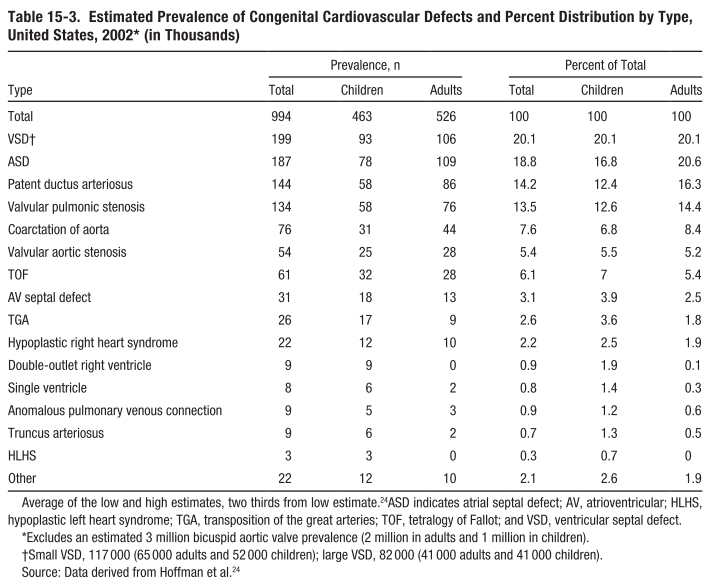
\includegraphics[width=0.6\textwidth]{5/chd-defects-usa.png}
\caption{Table of prevalences of congenital heart defects borrowed temporarily from \cite{Mozaffarian2016}.}
\label{ch5:fig:usa-defects-prev}
\end{figure}

CHD consists of a variety of defects which can affect any combination of the vessels and chambers of the heart with varying degrees of severity. The defects prevent the cardiopulmonary system as a whole from functioning correctly, but pinpointing and treating the defects effectively can be a complex process. It is important to note that each defect type has a different prevalence, a different treatment plan, and different expected outcomes. A breakdown of prevalence rates of some of the most common lesion types can be seen in Figure \ref{ch5:fig:usa-defects-prev}. % See (16)

% Causes of CHD: genetic syndromes, single gene mutations, environmental exposure, and unknown
Different presentations of CHD are associated with a number of different genetic and environmental factors \cite{Mozaffarian2016}. Genetic conditions such as Down syndrome, Turner syndrome, 22q11 deletion syndrome, Williams syndrome, and Noonan syndrome are associated with certain CHD presentations. Maternal behaviors such as smoking and binge drinking are known to cause heart problems in the fetus. Other maternal risk factors are obesity, folate deficiency, and living at a high altitude. Paternal exposure to phthalates, anesthesia, sympathomimetic medications, pesticides, and solvents may increase the risk of the fetus for developing CHD. While there are quite a few factors in this list, there are many CHD cases whose causes are unknown.

Once a patient is diagnosed with one of these defects or a cause of the CHD is identified, the specific nature of his case must be clearly documented. The documentation of CHD using the International Classification of Diseases, Ninth Revision, Clinical Modification (ICD-9-CM) has 25 high level codes representing various presentations of CHD, but these codes used alone are often not sufficient for describing a patient's true condition \cite{Mozaffarian2016}. Additional ICD-9-CM codes should be used to communicate the finer details of a patient's condition, if they are available. %something about how ICD codes make it easier to

The incidence of CHD in live births vary across countries and continents. The United States reports approximately 4-10 CHD case per 1000 live births. Europe and Asia see about 6.9 and 9.3 CHD cases per 1000 live births, though smaller studies have been conducted in many countries to measure local prevalence \cite{Mozaffarian2016}. In China, the incidence of CHD ranges from 8.98 to 11.1 per 1000 live births \cite{Zhao2019} \cite{Qu2016}. 
A pair of studies from Iran report incidences of 8.6 and 12.3 per 1000 live births, though the studies note that they were performed in different geographical locations with different populations within the country \cite{Nikyar2011} \cite{Rahim2008}.
One report from Dharan reports an incidence of 5.8 per 1000 patients admitted to a tertiary care hospital over a 12 month period \cite{Shah2008}. A study of newborns at one hospital in New Delhi, India claims an incidence of 3.9 per 1000 live births, though this rate may be a poor estimate as there is a significant delay between patient birth and referral to a cardiac center in India \cite{Khalil1994} \cite{Saxena2005}.

These incidence rates should be analyzed with some caution. In many cases, the reported rates were based on medical records. Medical records are not always correct; it is well known that human error can lead to a medical record lacking information or containing incorrect information. The only way for a person to have a medical record is for him or her to go to a medical center. Not everyone who has CHD is able to seek medical help, often because of their geographical locations or their income. Even if a patient is able to seek medical help, the availability of proper cardiac care varies between and within countries. However, it is generally expected that CHD incidence rates will increase as screening tools and treatments become more effective and more widespread, leading to earlier detection of defects.
 
% Diagnosis
Currently, the process of detecting and diagnosing CHD can begin before birth. A specialized ultrasound test called fetal echocardiography can detect heart abnormalities as early as the second trimester of the pregnancy. People who learn they are pregnant with a fetus who shows signs of CHD may choose to handle this information by opting for termination or pursuing a more detailed diagnosis. Additional tests, such as amniocentesis and follow-up ultrasounds may be used to determine treatment options before the patient is born. Generally, severe CHD cases present and are detected at earlier stages of life, but minor defects may not become apparent until the patient is older. Tests used to diagnose CHD in postnatal patients include electro- and echo-cardiograms, chest x-rays, pulse oximetry, exercise stress tests, computed tomography or MRI scans, and cardiac catheterization. Treatment of different defects varies from monitoring and medication to surgery and cardiac implants.

\begin{figure}
\centering
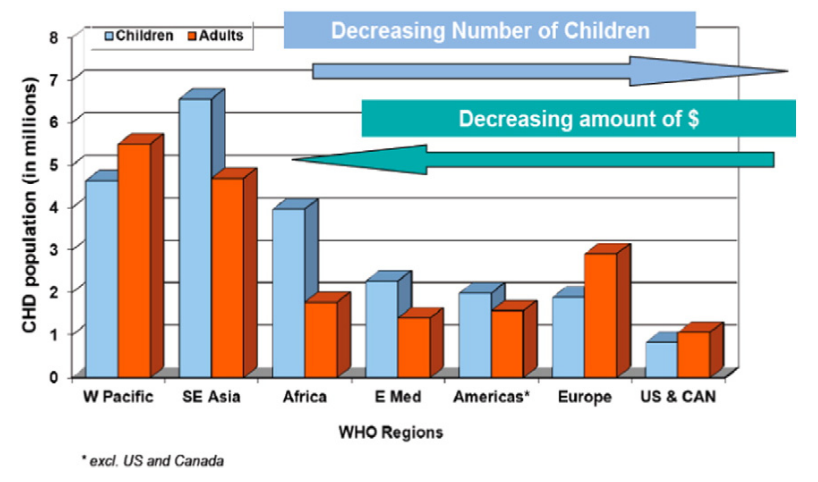
\includegraphics[width=0.7\textwidth]{5/CHD-burden-webb.png}
\caption{Estimated CHD burden in World Health Organization (WHO) regions using incidence rates of approximately 12/1000 and 4/1000 in children and adults, respectively \cite{Webb2015}.}
\label{ch5:fig:CHD-burden}
\end{figure}

%Depending on the cause of the 
The cost of diagnostic techniques and treatment plans impose different levels of financial burden on CHD patients and their families. Certain defects require complex, expensive surgical repairs while others can be treated with less expensive approaches \cite{Mozaffarian2016}. The burden of CHD across the globe was outlined by Webb et al \cite{Webb2015}. Their figure illustrating the prevalence of CHD and the availability of funds with which to treat it can be see in Figure \ref{ch5:fig:CHD-burden}. As the overall mortality of CHD declines, the burden of CHD is expected to increase \cite{Mozaffarian2016}.

% Complications and risks
Unfortunately, the cost of treating CHD is not the only burden a patient must undergo. Patients with CHD are also at increased risk for heart failure and infections \cite{Mozaffarian2016}. Children with CHD are at 19-fold risk for stroke compared to their healthy counterparts \cite{Fox2015}. In a study of Swedish citizens born between 1970 and 1993, Giang et al compared the prevalence of cardiac conditions in patients with and without CHD \cite{Giang2018}. They found that patients who had a CHD diagnosis were at about eight times higher risk for intracerebral hemorrhage and subarachnoid hemorrhage than their non-CHD counterparts. The CHD patients were also more likely to suffer from arrhythmia and heart failure. 

% When are patients diagnosed?
% Expected lifespan
% Treatment plan
% Financial burden

However, cardiac conditions are not the only complications CHD must deal with. Many of these patients also suffer from neurocognitive disorders that co-occur with CHD. Early research in this area focuses on the neurodevelopmental status of neonatal patients pre- and post-surgical intervention. One theory was that some factor or factors in the surgical intervention caused brain injuries in the patients. This idea proved to be inaccurate when researchers began detecting neurological malformations \textit{in utero}.

In a systematic review of available literature regarding prenatal and postnatal presurgical CHD cases and neurodevelopmental outcomes, Mebius et al. identify two theories about the causality of  neurodevelopmental delays and CHD \cite{Mebius2017}. The first theory is that abnormalities in the cardiac system prevent the developing brain from receiving enough oxygen and nutrients, which disrupts prenatal brain development. The second theory is that faulty genetic pathways used during both cardiac and brain development cause both conditions to co-occur. However, 11 articles Mebius et al. found during their review that are related to bloodflow through the umbilical artery suggest a third theory. During the prenatal period, a fetus receives oxygen from the mother via the placenta. If the placenta was not functioning correctly, it could lead to the fetus receiving not enough oxygen. Lower quantities of oxygen throughout prenatal development could potentially cause problems both in brain and cardiac growth. The 11 articles have contradictory results, but some researchers are currently investigating the role of the placenta in CHD and prenatal brain development.

Survival of CHD patients to adulthood has increased from 10\% to 90\% over the last several decades as CHD diagnostic tools and treatments have improved.  Currently, Webb et al. estimate that at least 12 to 34 million adults have CHD, and this number is expected to increase \cite{Webb2015}. The impact of the combination of CHD and neurological conditions throughout a patient's lifetime is starting to be explored. The aging of the CHD population has also sparked interest in the relationships between CHD and adult-stage neurological disorders such as dementia and Alzheimer's. 

While the purpose of this study is not to focus on CHD patients, we chose to use CHD and aging brain images in support of research being performed in the area of relationships between CHD and neurodevelopment.

%To address:
%\begin{itemize}
%\item Common combinations
%\item Joint treatment?
%\item Additional risks?
%\item Joint financial and emotional burden on caretakers? 
%\item CHD, neuro, and aging? Dementia/Alzheimer's? Recent data ... MIND neuroimaging ancillary r01 dec 17
%\end{itemize}


\subsection{Identifying Neurocognitive Disorders}

Neurocognitive disorders are usually diagnosed using at least one of many psychological survey-based evaluations, but these methods are subjective. rs-fMRIs could be used to identify patients who have functional connectivity patterns associated with different neurocognitive disorders, and eventually may be used to identify patients who are at risk for developing these disorders.

\subsubsection{Patient Surveys}

Surveys known to be used for studying the relationship between CHD and neurodevelopment are

\begin{itemize}
\item National Institute of Health Toolbox (3 - 85 years): ``Performance tests of cognitive, motor, and sensory function and self-reported measures of emotional function for adults and children in the general population and those living with a chronic condition''.

\item Sue Beers (4 - 18 years [not inclusive of 18 years]): WASI-II, NEPSY-2, WRAML-2, D-KEFS, WISC-IV, Grooved Pegboard, BRIEF, Beery-Buktenica VMI, ASRS, Conners-3, BASC-II, ABAS-II, PedsQL General, PedsQL Cardiac, Pictoral Scale Self Perception Profile.

\item SVR-III NDT (9 - 13 years [not inclusive of 13 years]): WIAT, NEPSY, WRAML, D-KEFS, WISC-V, Grooved Pegboard, BRIEF, Beery-Buktenica VMI, ASRS, Conners ADHD Index, BASC-II, ABAS-3, PedsQL General, PedsQL Cardiac

\item Bayley Scales of Infant and Toddler Development -III (1 - 24 months): Subtests include cognitive, language, social-emotional, motor, and adaptive behavior tests \cite{Mebius2017}.

\item Battelle Developmental Inventory (Birth - 8 years [not inclusive of 8 years]): Subsets include cognition, communication, social-emotional development, physical development, and adaptive behavior.

\item Developmental Assessment of Young Children (Birth - 6 years [not inclusive of 6 years]): Subtests include cognition, communication, social-emotional development, physical development, and adaptive behavior.

\item Preschool Language Scale + Receptive-Expressive Emergent Language (Birth - 3 years): Total language, auditory comprehension, expressive communication, articulation, receptive language, expressive language, and inventory of vocabulary words.

\item Peabody Developmental Motor Scales (Birth - 5 years): Subtests include reflexes, stationary, locomotion, object manipulation, grasping, visual-motor integration
\end{itemize}

The goal of these surveys is to compare the patient's cognitive function and neurological functions to expected milestones. Certain deviations from certain milestones are indicative of different disorders.

\subsection{Study Cohorts}

The rs-fMRIs used in this study were gathered as part of ongoing studies of the relationship between CHD and neurodevelopment. Data from the CHD/neurodevelopment studies was obtained through studies approved by the IRB at the Children's Hospital of Pittsburgh of UPMC and the University of Pittsburgh. All data is stored and accessed in compliance with HIPPA policies.

The subjects included in this analysis fall into three age groups: neonatal, preadolescent, and fetal. To summarize the cohorts, there were 163 brain rs-fMRIs obtained for the neonatal cohort, 546 brain rs-fMRIs obtained for the preadolescent cohort, and 124 brain rs-fMRIs obtained for the fetal cohort. The fetal cohort also contains 106 rs-fMRIs of the placenta. The race, ethnicity, and gender counts for these three cohorts can be seen in Figures  In the following sections, we describe each cohort in detail. 

\begin{figure}
\centering
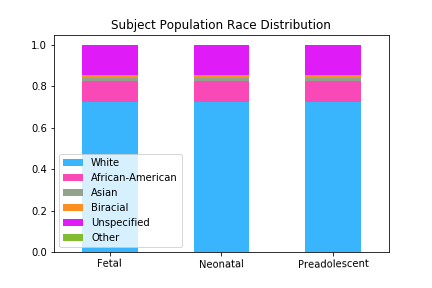
\includegraphics[width=.75\textwidth]{5/demo_clinical_subj_race.png}
\caption{Distribution of subject races for all three cohorts.}
\label{ch5:clinical:race}
\end{figure}%
%
\begin{figure}
\centering
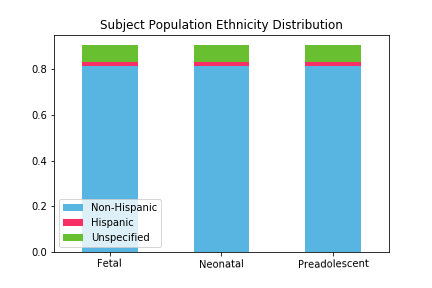
\includegraphics[width=.75\textwidth]{5/demo_clinical_subj_ethnicity.png}
\caption{Distribution of subject ethnicities for all three cohorts.}
\label{ch5:clinical:eth}
\end{figure}

\begin{figure}
\centering
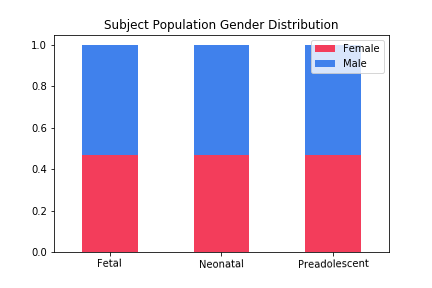
\includegraphics[width=.75\textwidth]{5/demo_clinical_subj_gender.png}
\caption{Distribution of subject genders for all three cohorts.}
\label{ch5:clinical:gender}
\end{figure}

\subsubsection{Neonatal Cohort and Images}

Neonatal subjects have been recruited as part of a prospective observational study. This cohort was scanned at two sites. At Site 1, the subjects were scanned using either a 3T Skyra (Siemans AG, Erlangen, Germany) or a 3T GE . At Site 2, the subjects were scanned using a 3T Philips (*).

The subjects were unsedated during the scans and a ``feed and bundle'' protocol was used to prevent motion during the scans \cite{Windram2011}. The newborns were positioned in the coil to minimize head tilting. Newborns were fitted with earplugs (Quiet Earplugs; Sperian Hearing Protection, San Diego, CA) and neonatal ear muffs (MiniMuffs; Natus, San Carlos, CA). An MR-compatible vital signs monitoring system (Veris, MEDRAD, Inc. Indianola, PA) was used to monitor neonatal vital signs. All scans were performed using a multi-channel head coil. The parameters for the resting-state BOLD MR scans were FOV=240 mm and TE/TR=32/2020 ms with interplane resolution of 4x4 mm, slice thickness of 4 mm, and 4 mm space between slices. The acquired images contained 150 volumes where each volume consisted of 64x64x32 voxels$^3$.

\begin{figure}
\centering
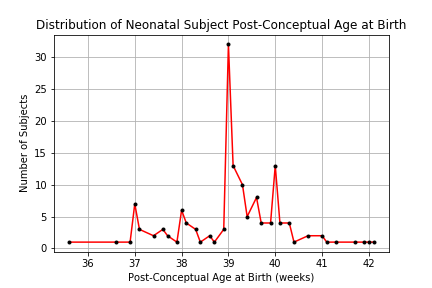
\includegraphics[width=.75\textwidth]{5/demo_neonate_subj_pca.png}
\caption{The distribution of post-conceptual ages at birth of all neonatal subjects.}
\label{ch5:neonates:birthpca}
\end{figure}

\begin{figure}
\centering
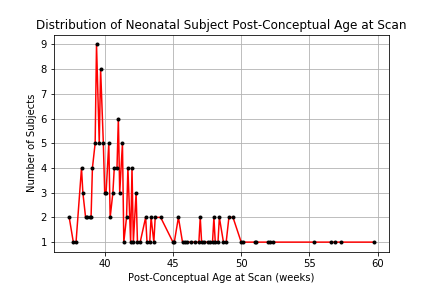
\includegraphics[width=.75\textwidth]{5/demo_neonate_scan_pca.png}
\caption{The distribution of post-conceptual ages at the time of the scan of all neonatal subjects.}
\label{ch5:neonates:scanpca}
\end{figure}

A total of 149 patients were recruited. The average post-conceptual age of the patients at birth was 39.08 weeks and they were on average 42.64 weeks post-conception at the time of the scan. The distribution of post-conceptual ages of the subjects at birth and at the time of the scan can be seen in Figure \ref{ch5:neonates:birthpca} and Figure \ref{ch5:neonates:scanpca}. 

\begin{figure}
\centering
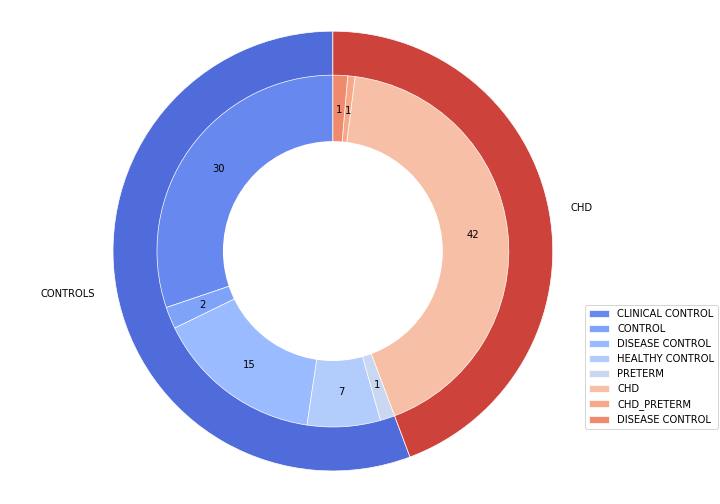
\includegraphics[width=1.0\textwidth]{5/demo_neonate_subj_cohort.png}
\caption{The breakdown of subject groups contained in the Control and CHD neonatal cohorts.}
\label{ch5:neonates:cohorts}
\end{figure}

The subjects were a mix of control subjects and CHD subjects. A comprehensive breakdown description of the subgroups within these two cohorts can be seen in Figure \ref{ch5:neonates:cohorts}. In this figure, the term ``Control'' encompasses both healthy full-term subjects, healthy pre-term subjects, and non-CHD clinical subjects (clinical control and disease control). The CHD group is composed of subjects diagnosed with CHD who were either born full-term or pre-term. Of the entire cohort, 14 subjects underwent two scanning sessions resulting in 163 rs-fMRI scans.

As the neonates were most often asleep during the scan, they exhibit less motion overall compared to our other clinical cohorts. The high-motion neonates are an obvious exception to this concept, but many of the high-motion images contained long periods where the subject was stationary. Applying both the DAG-based framework and the traditional registration framework to these images provided the opportunity to compare the performances of both registration frameworks to each other in the context of the usability gold standard thresholds. 

\subsubsection{Preadolescent Subject Population and Images}

As part of a multicenter study of CHD in preadolescents, we collected rs-fMRIs from nine sites throughout the United States. These images were of patients in the age range of 9 to 13 years who either had CHD or were healthy with no neurocognitive impairments. In addition to the MRI scans, subjects who participated in this study were asked to participate in additional testing  either to determine their neurocognitive outcome status or to perform genetic analyses. % (GET DETAILS FROM NANCY).

\textbf{Preadolescent Cohort.} The multicenter imaging study of preadolescent subjects provides a unique opportunity to evaluate the efficacy of the DAG-based framework on a large subject cohort containing variable amounts of motion. The outcome of this experiment will be used in the next experiment to determine if there are any site-specific or vendor-specific variables influencing patient motion.

%\begin{itemize}
%\item How were the images gathered?
%\item How were the patients recruited?
%\item What are the imaging protocol details?
%\item What other information was collected?
%\end{itemize}

\subsubsection{Fetal Subject Population and Images}

%Real goal is to develop a method of registering fetal brain and placental images so that we can further examine the relationship between placental oxygen levels and fetal brain development. Longitudinally, this technique can be used to determine how placental oxygen flow and fetal brain development impact a patient over the course of his or her life. Once the relationship between the placenta and fetal brain development is better understood, we can determine a set of neuroprotective interventions to employ for at-risk patients before they are born.

Fetal subjects have different constraints on their physical environment than neonates, preadolescents, and adults. As a result, they exhibit unique patterns of motion. The previous subject cohorts discussed in this chapter have the following commonalities: the subject experiences the full effects of gravity, the subject is lying on his back in an MRI scanner, and the subject's head motion is limited by the head coil within the MRI. Any motion in these images is a direct result of the subject himself moving, whether passively (cardiac motion and breathing) or actively (fidgeting or looking around).

A fetal subject is scanned in vivo. He is suspended in amniotic fluid within his mother. The amniotic fluid has buoyancy that reduces the effects of gravity and allows a fetal subject significant freedom of movement. The fetus can rotate, shift, and flip in ways that can only be accomplished when floating in a body of water. The properties of the uterus constrain the physical space in which a motion could occur, but not as much as the head coil and gravity do to the other patient cohorts. A fetus is not guaranteed to be in any specific position at the start of the scan: the scan begins when the mother is ready, not when the fetus achieves a certain pose. 

The fetal subjects underwent fetal echocardiography scans in a cardiac clinic to determine whether they were healthy or had a form of CHD. They were then scanned on an MRI scanner. Images of the fetal brain and the placenta were acquired for each subject. 

We are interested in both the fetal brain and placental images for our work because of the relationship between placenta and brain development. However, these organs have very different physical properties. The fetal brain is a rigid structure floating and moving within the amneotic fluid. It undergoes translation and rotation as a single unit due to passive and active maternal and fetal motions. The placenta, on the other hand, is anchored in place on the uterine wall. It may undergo small translations or rotations due to maternal motion, but it will respond differently to fetal motion. Fetal motions cause nonlinear deformations of the pliable placenta that can only be adequately accounted for using nonlinear registration algorithms. Nonlinear registrations have the potential to deform brain images into physically impossible shapes, so the fetal brain and placenta were manually segmented in their respective images so that each organ could undergo independent motion correction. 

The segmenters were one of a group of four researchers. While one researcher trained the other three group members, the interrater agreement between them is still being determined.

As the fetal subjects have both neurological and placental images, their data will be used to examine the impact of volume registration on different organ types.


%\begin{itemize}
%\item Fetal patients scanned between XX and XX weeks gestational age. 
%\item Imaging protocol details?
%\item What other information is collected about fetus and/or mom?
%\end{itemize}

\subsubsection{Aging Brain Subjects}

The ADNI study was launched in 2003 as a public-private partnership, led by Principal Investigator Michael W. Weiner, MD. The primary goal of ADNI has been to test whether serial magnetic resonance imaging (MRI), positron emission tomography (PET), other biological markers, and clinical and neuropsychological assessment can be combined to measure the progression of mild cognitive impairment (MCI) and early Alzheimer's disease (AD). For up-to-date information, see www.adni-info.org.

%\begin{itemize}
%\item How were the images gathered?
%\item How were the patients recruited?
%\item What are the imaging protocol details?
%\item What other information was collected?
%\end{itemize}

%The second adult cohort comes from the Alzheimer's Disease Neuroimaging Initiative (ADNI) dataset. The ADNI study has been working since 2004 to further Alzheimer's research by gathering, analyzing, and sharing clinical, imaging, genetic, and biochemical biomarkers from the elderly population. The group gathers data from 63 sites in the United States and Canada. During the second phase of the study, sites who have a Philips MRI system gathered resting-state fMRIs from their subjects. This data is freely available to academic researchers through the LONI Image and Data Archive.

The adult cohort encompass many clinical outcomes and a wider age range than the other clinical populations. The adult cohort also allows for another opportunity to study a different type of motion patterns associated with the aging brain rather than the still-developing brain.

\subsection{Summary}
%ELEPHANTS 3-5 sentences about CHD here

While we have amassed a large collection of clinical images, an analysis of purely clinical images is not sufficient in determining which volume registration technique recovers more brain signal. In the next section, we elaborate on this limitation and how we chose to address it.

\section{Simulated Sequences} % ELEPHANTS should this be its own chapter?

There are two major barriers in research surrounding motion correction in rs-fMRIs: gathering data and measuring the effects of the technique. In this section, we elaborate on a simulation designed to address both of these barriers.

\subsection{Background}

Despite the hundreds of images in each of the patient populations described in the previous section, our clinical data would be considered too sparse for ``big data'' analyses. This problem is not unique to our group: it is difficult to obtain enough data from a large number of subjects to perform large-scale studies. Collaborators can band together to create a larger and more diverse data set by participating in multicenter studies. There are some challenges associated with multicenter studies. Each site will have a different scanner, potentially with different field strengths and from different manufacturers. Even ignoring the challenges of harmonizing data obtained using scanners from different companies, each scanner has its own set of unique inhomogeneities in the primary magnetic field. Additional scans of inanimate or human phantoms may be necessary to characterize the differences between all of the scanners involved.

The second barrier to motion correction in rs-fMRI research is the complexity of identifying a gold standard metric to use when evaluating motion correction techniques. The current gold standard metrics developed by Power et al. evaluate motion correction techniques in terms of the reduction of positional differences and signal differences between neighboring volumes. Unfortunately, this approach does not measure the amount of signal recovered or lost though motion correction. A true gold standard evaluation of motion correction would be able to evaluate the BOLD signal present in the image before and after correction. If the BOLD signal prior to patient motion was known, though, there would be no need for image processing in the first place: we would already have the data we are trying to obtain with motion correction.

We address these two barriers by creating a mechanism for generating simulated image sequences. The generated sequences contain simulated brain signal based in areas of the brain associated with resting-state connectivity, scanner noise, and patient motion. Our mechanism can create large quantities of unique image sequences. The simulated image sequences can also serve as a gold standard for evaluating volume registration and motion correction techniques: the signals and noise sources added to the sequence are known with certainty.

%Every MRI scanner is different, even those made by the same manufacturer. To ensure MRI scans obtained from different scanners are comparable.  so a stand-in model for an organ or tissue type is often used to calibrate an MRI scanner. The model is designed to have specific physical properties which mimic the physical properties of the organ or tissue. These properties can be accurately measured during the design process of this model so that the radiologist or researcher looking at images of the model can know the ground truth of the model. Because these models mimic true organs and tissues, they are called phantoms. 

\subsection{SPECTr: Simulated Phantom Emulating Cranial Transformations}

Our mechanism is called Simulated Phantom Emulating Cranial Transformations (SPECTr). A phantom is an object designed to have material properties which mimic those of a specific tissue type or organ. Phantoms, either manufactured objects or healthy humans, are used in multicenter studies to obtain images of the same object or person from multiple scanners. These images are used to harmonize the data taken from the different sites. We call our simulated sequence a phantom because the baseline image itself is known as are the signals added to it to simulate brain activity. 

% ELEPHANTS
When developing the pipeline for SPECTr, it was important to consider the effects of motion and various impacts they have on the BOLD signal. As discussed in CHAPTER, the three effects of motion are positional, spin history, and susceptibility. For simplicity, we combine the spin history and susceptibility effects into ...

\subsection{Materials}

In order to simulate resting-state BOLD signal in an fMRI, two pieces of anatomical information are required. The first is structural information about the brain. The second is the location of functional networks associated with the resting-state BOLD signal.

While it is possible to use clinical images for the structural information, the goal of SPECTr is to be generalizable both for our use and for the use of other researchers. Additionally, clinical images inherently contain some degree of signal from some neuronal processes which could obfuscate the simulated BOLD signal. 

In 1992, the International Consortium for Brain Mapping was formed to develop as set of standards for what is considered a healthy human brain. They used their criteria to develop an initial set of ``average'' brain structural scans based on scans from healthy volunteers. This original set of average brain scans incorporates scans from 305 subjects and is referred to as the MNI305 data. As MRI technology has evolved, the spatial resolution capabilities of the MRI scanners has increased. In 2001, another set of 152 healthy volunteers was recruited to create a higher resolution data set. The scans from the new cohort were linearly registered to the MNI305 data to create the new MNI152 images. % ELEPHANTS citations needed

Herein, we use the MNI152 data set as available at the website for the McConnell Brain Imaging Centre at McGill University. This data set contains five images: a T1-weighted scan, a T2-weighted scan, a proton density weighted scan, and two binary masks for the head and the brain. Each of the structural scans was designed to highlight the properties of different tissues in and around the brain. Proton density scans were developed for the purpose of detecting blood-related signal. As BOLD images essentially perform the same purpose over a period of minutes, we choose to use the proton density weighted scan as the structural base for the simulated images. % ELEPHANTS citations needed

The functional network information is more difficult to find than structural atlases. The Functional Imaging in Neuropsychiatric Disorders Lab at Stanford has developed two sets of functional atlases. The atlases are divided into regions of interest (ROIs) associated with individual networks. The first set of atlases contains 90 functional ROIs which compose 14 networks. The second set of atlases contains 499 functional ROIs and has more gray matter coverage. For simplicity, we chose to use the original ROIs associated with the dorsal and ventral default mode networks.

\subsection{Simulation Pipeline}

\subsubsection{Baseline Sequence}

\begin{figure}
\centering

\includegraphics[width=.5\textwidth]{5/pipeline.png}
\caption{An overview of the SPECTr simulation pipeline. Using atlas data, a simulated phantom containing brain signal, scanner noise, and patient motion is generated.}
\label{ch5:spectr_flow}
\end{figure}

The process for generating a simulated sequence using the data discussed in the previous section has several steps. An overview of the pipeline can be seen in Figure \ref{ch5:spectr_flow} We cover these steps in detail in this section.

The MNI152 proton density image is a whole head image. To remove the skull, we apply the brain mask to the proton density weighted image. The resulting image contains only brain tissue.

The spatial resolution of the structural brain image is 1 mm$^3$. The spatial resolution for a single volume in a rs-fMRI sequence is less granular at 4mm$^3$. To achieve this resolution, the structural volume must be downsampled. After the downsampling, the size of the structural image is reduced from 181x217x181 voxels to XXxXXxXX voxels. %ELEPHANTS interpolation?

Now that the structural image is the correct spatial resolution, it must be replicated to create the temporal sequence. Part of this step includes creating a new dimension in the data. The affine matrix which represents the resolution of the image has the following structure:

\begin{equation}
\begin{bmatrix}
 r_x &  0   &  0   & c_x\\ 
 0   &  r_y &  0   & c_y \\ 
 0   &  0   &  r_z & c_z \\ 
 0   &  0   &  0   & 1 
\end{bmatrix}
\end{equation}

\noindent where $r_x, r_y,$ and $r_z$ represent the spatial resolution in the $x, y,$ and $z$ axes, respectively and $c_x, c_y,$ and $c_z$ represent the location of the origin in voxels. To convert the image from a 3D volume to a 4D sequence, we add a row and a column to this matrix so that it now has the structure:

\begin{equation}
\begin{bmatrix}
 r_x &  0   &  0   & 0 & c_x\\ 
 0   &  r_y &  0   & 0 & c_y \\ 
 0   &  0   &  r_z & 0 & c_z \\ 
 0   &  0   &  0   & t & 0 \\
 0   &  0   &  0   & 0 & 1 
\end{bmatrix}
\end{equation}

\noindent where $t$ is the desired temporal resolution. We choose a temporal resolution of 2 seconds for our simulated sequence. The downsampled image volume is replicated and concatenated along the new temporal dimension to create a sequence that is 150 image volumes long. This sequence is referred to as the base phantom sequence as it contains no brain signal, noise, or motion.

\subsubsection{Brain Signal}

The next step in the pipeline is to add BOLD signal to the sequence. % ELEPHANTS (Why brain signal next?) 
We combine the functional ROIs from the dorsal and ventral default mode networks into a single binary functional ROI image. This image is referred to as the default mode network (DMN) mask. 

For each nonzero voxel in the DMN mask, a temporal signal is generated. We chose to model the BOLD response as a cosine signal following the formula

\begin{equation}
s(\vec{v}, t) = a*(cos(f_0 * (t-t_{shift})) - a_shift).
\label{ch5:bold_eq}
\end{equation}

\noindent This equation is for a scaled cosine function with both temporal and amplitude shifts. The temporal and amplitude shifts, $t_{shift}$ and $a_{shift}$ respectively, are randomly generated for each voxel from uniform distributions. Once chosen, they are consistent across the voxel's generated temporal signal. The other parameters, $a$ and $f_0$, were specified using existing research. 

In 2007, Biswal et al. performed a study evaluating methods to reduce changes in the BOLD signal not directly related to brain activity (i.e., vascularity). They identified a low-frequency spectral amplitude of 0.04 Hz as the highest frequency related to BOLD signal consistent not only through scans of individual patients but in group-wise analyses. Based on their work, we chose the fundamental frequency $f_0$ to be 0.04 Hz. % ELEPHANTS citation

The scaling factor $a$ was chosen based on Power et al.'s usability criteria. As they state that any signal change between volumes above 2.5\% of the maximum voxel value is unlikely to be due to brain activity, we used an amplitude of 20 units on a scaled voxel value range of [0, 1000]. % ELEPHANTS citation

The generated BOLD signals were added to the baseline image sequence, but were also saved in a separate image sequence file for reference during analysis. The generated sequence with only BOLD signal is referred to as the brain signal sequence.

\subsubsection{Scanner Noise}

The next step in the pipeline is to add scanner noise to the brain signal sequence. In a regular rs-fMRI of a patient, the noise in the sequence is the result of two factors: the spin history effects of motion and the susceptibility effects of motion. To simplify the simulation, we choose to model the resulting noise rather than the individual sources.

Signal acquired by MRI scanners is first recorded as a raw data matrix in k-space. K-space contains spatial frequency information. The coordinate system of k-space differs from the coordinate system of physical space. In k-space, the closer a point is to the center of a zero-centered data matrix, the lower its frequency or phase. The brighter a point in the raw data matrix is, the larger its magnitude. 

While frequency is a continuous spectrum, data is usually divided into low frequency data and high frequency data. Low frequency data in imaging is areas of an image where the pixel or voxel values slowly. In physical space, these areas are the smooth areas that contain content. In Figure REF, the skin on the woman's face would be considered low frequency data. High frequency data represents the areas in an image where the pixel or voxel values change rapidly in a small area. Areas with many edges in them contain higher frequency data. In Figure REF, the feather in the woman's hat would be considered high frequency data. % Need a figure ELEPHANTS 

Generally speaking, images contain more low frequency information than high frequency information. We wish to be able to control the amount of noise added to each component independently, so we choose to add noise to the sequence in k-space.

When adding scanner noise to the brain signal sequence, we add noise to each image volume independently. The image volume is transformed from physical space into k-space using the fast Fourier transform (FFT). To force the image to be zero-centered, we perform a FFT shift on the Fourier space data. A matrix the same size and shape as the image volume is created. The matrix is then filled with complex Gaussian noise, $n(\vec{l})$ where

\begin{equation}
|n(\vec{l})| = w_m * r_m, r_m~N(0,1)
\end{equation}

\noindent and

\begin{equation}
\angle n(\vec{l}) = w_p * r_p, r_p~N(0,1)
\end{equation}

\noindent In these two equation, $\vec{l}$ is the location of the point in the matrix, $w_*$ represents the weight assigned to the component, $r_*$ represents the noise random variable independently generated from a standard normal distribution, and the subscripts $m$ and $p$ refer to the magnitude and phase components, respectively. The complex noise is weighted so that the magnitude of the noise has a greater contribution than the phase of the noise, that is $w_m > w_p$ 

The matrix of complex noise is added to the zero-centered k-space image volume. The noisy k-space volume is unshifted and undergoes an inverse Fourier transform to change the data back to physical space.

\subsubsection{Patient Movement}

Now that the ground truth brain orientation and BOLD signal have been established, patient motion can be added to the BOLD phantom sequence. One of the aims of this document is to establish that patients from different populations exhibit different motion patterns. As we have not yet established what those motion patterns are, we developed a generic motion model for the simulation.

During an rs-fMRI scan, a patient theoretically has the freedom to rotate his head around three different axes, translate his head along three different axes, or some combination of translations and rotations. Realistically, once a patient has settled in the scanner, it becomes difficult for his head to only undergo translation. It is more likely that he will rotate his head. For the simplicity of the simulation, we assume no head translations occur during the scan.

A rotational transformation can be represented as a matrix. Rotations about a single axis are represented as followed:

\begin{equation}
R_x(\alpha) = \begin{bmatrix}
 1 &  0          & 0     \\ 
 0 &  cos\alpha  & sin\alpha \\ 
 0 &  -sin\alpha & cos\alpha \\ 
\end{bmatrix}
\end{equation}
\begin{equation}
R_y(\beta) = \begin{bmatrix}
 cos\beta &  0 & -sin\beta \\ 
 0        &  1 & 0         \\ 
 sin\beta &  0 & cos\beta  \\ 
\end{bmatrix}
\end{equation}
\begin{equation}
R_z(\gamma) = \begin{bmatrix}
 cos\gamma  & sin\gamma  & 0 \\ 
 -sin\gamma & cos\gamma  & 0 \\ 
 0          & 0          & 1 \\ 
\end{bmatrix}
\end{equation}

Rotational transforms are applied to the origin of the image. However, the origin of the image is not necessary anatomically significant. Head motion naturally occurs about the base of the neck. We can approximate the location of the base of the neck by calculating the center of mass of the brain. First, the image volume is thresholded to separate the brain from the background. Then the locations of the ``on'' voxels are averaged to calculate the center of mass. 

Motion is added to the noisy image sequence one volume at a time. No motion is applied to the first volume in the sequence, but volume is used to calculate the center of mass of the brain. For each subsequent volume, the angles of rotation about the x-, y-, and z-axes are each randomly generated from a standard normal distribution to create rotational change matrices, $R_{*,\Delta}$ (where the subscript $*$ represents $x$, $y$, or $z$). The new rotations $R_{*,\Delta}$ are added to the rotations from the previous step $R_{*,i-1}$ to create the rotation matrices for the current volume, $R_{*,i}$:

\begin{equation}
R_{*,i} = R_{*,i-1} + R_{*,\Delta}
\end{equation}

The three rotational transformations are combined into one matrix via multiplication: 

\begin{equation}
R_i = R_{x, i}(\alpha) R_{y,i}(\beta) R_{z,i}(\gamma)
\end{equation}

The compound transformation $R_i$ is then applied to the image at the center of mass calculated from the original image volume. \textit{Note: Since the simulation is constrained by the assumption of no head translations, the center of mass will remain consistent throughout the image sequence.}

After motion has been added to every image volume in the sequence, the sequence with motion is ready to be used in motion correction analyses.

\subsection{Implementation}

SPECTr is implemented in Python (version 3.7.3). The \lstinline{nipy} library (version 0.4.1) was used to load images, save images, and combine the functional ROIs. The \lstinline{numpy} library (version 1.17.4) was used for matrix manipulations involved in the brain signal and noise generation steps. The image processing library \lstinline{skimage} (version 0.14.2) was used to calculate the center of mass. The Python wrapper \lstinline{SimpleITK} (version 1.2.4) of the Insight Toolkit library for image analysis was used to perform the rotational transformations associated with patient motion.

The source code for SPECTr is available on Github at \url{https://github.com/jmschabdach/SPECTr}.


%First, a reasonable range of head rotation about the x-, y-, and z-axes was established. These angle ranges are used to generate rotational transformation matrices for $N-1$ image volumes. The transformations are applied to each image volume after the first volume in the BOLD phantom sequence. The transformed image sequence is referred to as the BOLD phantom sequence with motion and the rotational transformation matrices are saved as the ground truth for the transformations between each image volume and the template volume. 
%The BOLD phantom sequence serves as the ground truth for any motion correction pipeline: it contains the known brain orientation and BOLD signal independent from head motion and scanner noise.

\subsection{Experiments Involving Simulated Images}

We generated 90 image sequences from the MNI152 proton density image and the default mode network functional ROIs using the process described in the previous section. The image sequences were divided into three groups with different degrees of scanner noise. All simulated images underwent both registration techniques described in Chapter \ref{ch:mri}. The registered images also underwent independent component analysis (ICA) using FSL's MELODIC (Multivariate Exploratory Linear Optimized Decomposition into Independent Components) tool. % ELEPHANTS SOURCES

The registered images will undergo the same type of analysis as the clinical images. The ICA technique will be used to determine how much brain signal was recovered by each registration technique.

This particular experiment will be one of the first to investigate how much true BOLD signal is preserved through motion correction. One of the major drawbacks to existing motion correction pipelines is that they remove signal along with noise. In clinical data, there is no way to know the ground truth signal contained within the image; however, simulated phantom images have a de facto known ground truth signal. The design for this experiment can be used to evaluate how much BOLD signal is recovered by other motion correction pipelines, and how close the recovered signal is to the signal of interest.

\section{Summary}

In this chapter, we discussed our three major data sets, which are drawn from simulated data, pediatric data, and aging brain data. The simulated data were generated using a rs-fMRI simulation pipeline developed in-house and were used for the purpose of measuring ground truth signal recovered by motion correction techniques. The pediatric data were obtained through prospective studies of CHD and neurodevelopment being conducted at the UPMC Children's Hospital of Pittsburgh. The pediatric and aging brain images were used to compare the two volume registration techniques in a standalone analysis as well as in the context of a motion correction pipeline. We also used these images to examine patterns of motion unique to different age groups. 
%\chapter{RESULTS}
\label{ch:results}

This chapter is divided into two main sections. The first section focuses on the comparison of the two motion correction techniques. The second section focuses on the results of the machine learning algorithms applied to the metrics extracted from the images.

Each of the clinical images underwent volume registration using both registration methods outlined in Chapter \ref{ch:moco}. The FD and DVARs metrics were calculated for every pair of subsequent volumes $i$ and $i+1$ in the original sequences, the traditionally registered sequences, and the DAG-registered sequences. Then the sequences were comprehensively compared to themselves. For every volume in each sequence, the Dice metric, the mutual information, and the correlation ratio were calculated for the volume and every other volume in the sequence.

The simulated data underwent the same analyses as the clinical images, with one addition. Independent component analysis was performed on the simulated data to identify components contributing to the overall signal in the image. By correlating the components with the simulated signal for each image, the BOLD-related components were identifies. The amount of BOLD signal identified for each image was compared to that image's original BOLD signal.


\section{Simulated Data}

\subsection{Volume Registration: Power Thresholds}

\begin{figure}[t]
	\centering
	\begin{subfigure}{0.4\textwidth}
		\centering
		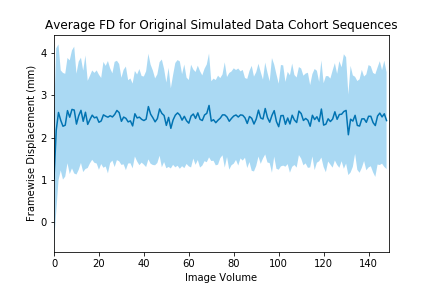
\includegraphics[width=1.0\textwidth]{6/figures/spectr-bold-fd-150.png}
		\caption{FD of Original Sequences.}
	\end{subfigure}
	\hspace{0.05\textwidth}
	\begin{subfigure}{0.4\textwidth}
		\centering
		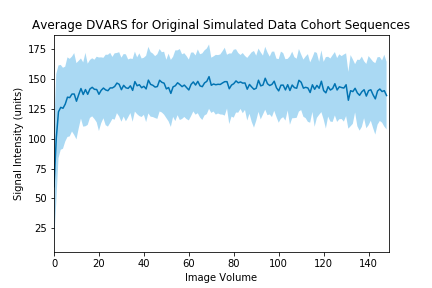
\includegraphics[width=1.0\textwidth]{6/figures/spectr-bold-dvars-150.png}
		\caption{DVARS of Original Sequences.}
	\end{subfigure}
	
	\begin{subfigure}{0.4\textwidth}
		\centering
		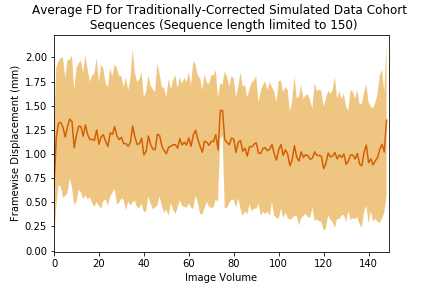
\includegraphics[width=1.0\textwidth]{6/figures/spectr-trad-fd-150.png}
		\caption{FD of Traditionally Registered Sequences.}
	\end{subfigure}
	\hspace{0.05\textwidth}
	\begin{subfigure}{0.4\textwidth}
		\centering
		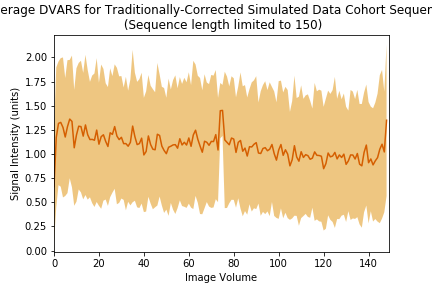
\includegraphics[width=1.0\textwidth]{6/figures/spectr-trad-dvars-150.png}
		\caption{DVARS of Traditionally Registered Sequences.}
	\end{subfigure}
	
	\begin{subfigure}{0.4\textwidth}
		\centering
		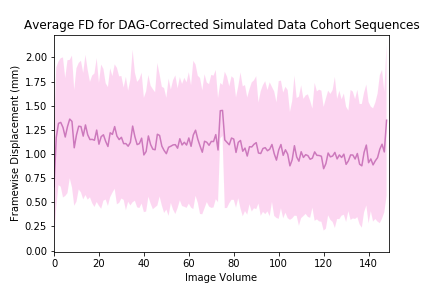
\includegraphics[width=1.0\textwidth]{6/figures/spectr-dag-fd-150.png}
		\caption{FD of DAG-Registered Sequences.}
	\end{subfigure}
	\hspace{0.05\textwidth}
	\begin{subfigure}{0.4\textwidth}
		\centering
		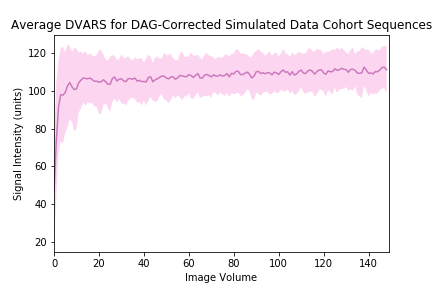
\includegraphics[width=1.0\textwidth]{6/figures/spectr-dag-dvars-150.png}
		\caption{DVARS of DAG-Registered Sequences.}
	\end{subfigure}
\caption{The means and standard deviations of the FD and DVARS metrics for all simulated images both before and after registration.}
\label{fig:neonate-power-dists}
\end{figure}

The FD and DVARS metrics were calculated between every pair of image volumes $i-1$ and $i$ for the original sequences and both types of registered sequences. The mean of the FD and DVARS metrics for each time point for each sequence type  can be seen in Figures

\begin{table}[h!]
\centering
\caption{The number and percentage of image volumes across all sequences in the simulated cohort which meet the usability thresholds of FD \textless 0.2 mm and DVARS \textless 2.5\%.}
\label{tab:spectr-power-thresh}
\begin{tabular}{|c|c|c|c|}
\hline
\textbf{Threshold Met} &
  \textbf{\begin{tabular}[c]{@{}c@{}}Original\\  Sequences\end{tabular}} &
  \textbf{\begin{tabular}[c]{@{}c@{}}Traditionally Registered \\ Sequences\end{tabular}} &
  \textbf{\begin{tabular}[c]{@{}c@{}}DAG-Registered \\ Sequences\end{tabular}} \\ \hline
FD (count)    & 98    & 329   & 279   \\ \hline
DVARS (count) & 54    & 53    & 53    \\ \hline
Both (count)  & 53    & 46    & 44    \\ \hline
FD (\%)       & 0.731 & 2.453 & 2.081 \\ \hline
DVARS(\%)     & 0.403 & 0.395 & 0.395 \\ \hline
Both (\%)     & 0.395 & 0.343 & 0.328 \\ \hline
\end{tabular}
\end{table}

Table \ref{tab:spectr-power-thresh} shows the number of and percentage of image volumes in all simulated image sequences which meet the FD threshold, the DVARS threshold, and both thresholds. Across all 90 image sequences, there were 150 image volumes per sequence bringing the total number of image volumes to 13,410 image volumes. In the original images, less than 1\% of the image volumes met the individual thresholds with only 0.395\% of image volumes meeting both thresholds. After either registration, over 2\% of the image volumes meet the FD threshold.

\begin{table}[h!]
\centering
\caption{Results from the t-tests comparing the counts for the numbers of images meeting the FD, DVARS, and FD and DVARS thresholds for sequence type $S_1$ and sequence type $S_2$.}
\label{tab:spectr-power-ttest}
\begin{tabular}{|c|c|c|c|}
\hline
\textbf{Sequence Type 1 ($S_1$)} &
  \textbf{Original} &
  \textbf{Original} &
  \textbf{\begin{tabular}[c]{@{}c@{}}Traditionally \\ Registered\end{tabular}} \\ \hline
\textbf{Sequence Type 2 ($S_2$)} &
  \textbf{\begin{tabular}[c]{@{}c@{}}Traditionally\\ Registered\end{tabular}} &
  \textbf{\begin{tabular}[c]{@{}c@{}}DAG\\ Registered\end{tabular}} &
  \textbf{\begin{tabular}[c]{@{}c@{}}DAG\\ Registered\end{tabular}} \\ \hline
\begin{tabular}[c]{@{}c@{}}P($S_1$ and $S_2$ have \\ same FD counts)\end{tabular} &
  1.05 E -16 &
  4.49 E -11 &
  0.127 \\ \hline
\begin{tabular}[c]{@{}c@{}}P($S_1$ and $S_2$ have \\ same DVARS counts)\end{tabular} &
  0.941 &
  0.941 &
  1.0 \\ \hline
\begin{tabular}[c]{@{}c@{}}P($S_1$ and $S_2$ have \\ same FD and DVARS counts)\end{tabular} &
  0.590 &
  0.486 &
  0.872 \\ \hline
\end{tabular}
\end{table}

To determine the statistical significance of these differences, a series of independent 2 sample t-tests were performed. For each test, two types of sequences were chosen. The distributions of samples were the numbers of image volumes in each sequence meeting the usability threshold of interest. The null hypotheses for the t-tests were that the number of volumes meeting the threshold for each sequence type were the same and the alternative hypothesis was that this number was different. The results of these tests can be seen in Table \ref{tab:spectr-power-ttest}. The only statistically significant differences were for the number of image volumes meeting the FD threshold. The counts for the registered images each differed from the original images at $p < 0.005$ while the difference between the two registrations was not significant ($p = 0.127$).

\begin{table}[h!]
\centering
\caption{The number of subjects whose sequences of types $S_1$ and $S_2$ had different FD distributions.}
\label{tab:spectr-fd-kstest}
\begin{tabular}{|c|c|c|c|}
\hline
\textbf{\begin{tabular}[c]{@{}c@{}}\# Sequences \\ Type 1 ($S_1$)\end{tabular}} &
  \textbf{\begin{tabular}[c]{@{}c@{}}\# Sequences \\ Type 2 ($S_2$)\end{tabular}} &
  \textbf{\begin{tabular}[c]{@{}c@{}}\# Sequences \\ p \textless 0.05\end{tabular}} &
  \textbf{\begin{tabular}[c]{@{}c@{}}\# Sequences \\ p \textless 0.005\end{tabular}} \\ \hline
Original                                                            & \begin{tabular}[c]{@{}c@{}}Traditionally\\ Registered\end{tabular} & 90 & 90 \\ \hline
Original                                                            & \begin{tabular}[c]{@{}c@{}}DAG\\ Registered\end{tabular}           & 90 & 90 \\ \hline
\begin{tabular}[c]{@{}c@{}}Traditionally \\ Registered\end{tabular} & \begin{tabular}[c]{@{}c@{}}DAG\\ Registered\end{tabular}           & 40 & 27 \\ \hline
\end{tabular}
\end{table}

\begin{table}[h!]
\centering
\caption{The number of subjects whose sequences of types $S_1$ and $S_2$ had different DVARS distributions.}
\label{tab:spectr-dvars-kstest}
\begin{tabular}{|c|c|c|c|}
\hline
\textbf{\begin{tabular}[c]{@{}c@{}}\# Sequences \\ Type 1 ($S_1$)\end{tabular}} &
  \textbf{\begin{tabular}[c]{@{}c@{}}\# Sequences \\ Type 2 ($S_2$)\end{tabular}} &
  \textbf{\begin{tabular}[c]{@{}c@{}}\# Sequences \\ p \textless 0.05\end{tabular}} &
  \textbf{\begin{tabular}[c]{@{}c@{}}\# Sequences \\ p \textless 0.005\end{tabular}} \\ \hline
Original                                                            & \begin{tabular}[c]{@{}c@{}}Traditionally\\ Registered\end{tabular} & 90 & 90 \\ \hline
Original                                                            & \begin{tabular}[c]{@{}c@{}}DAG\\ Registered\end{tabular}           & 90 & 90 \\ \hline
\begin{tabular}[c]{@{}c@{}}Traditionally \\ Registered\end{tabular} & \begin{tabular}[c]{@{}c@{}}DAG\\ Registered\end{tabular}           & 3  & 0  \\ \hline
\end{tabular}
\end{table}

For a more general comparison, the FD and DVARS metrics for each subject were compared for each type of registration. These distributions of FD and DVARS values for the original, traditionally registered and DAG-registered sequences underwent pairwise comparisons using the Kolmogorov-Smirnov test which evaluates the difference between two probability distributions. 

Table \ref{tab:spectr-fd-kstest} shows the number of comparisons between each sequence type where the Kolmogorov-Smirnov test produced a p-value less than 0.05 and 0.005 for the FD metrics. This table shows that the all images registered using either type of registration had significantly different FD distributions than the original images. It also shows that the traditionally registered and DAG-registered sequences had significantly different FD distributions with $p < 0.05$ for almost half (40/90) of the sequences and $p < 0.005$ for almost a third (27/90) of the sequences.

Table \ref{tab:spectr-dvars-kstest} shows similar results for the DVARS metrics of the registered and original sequences. However, only 3/90 of the registered image sequences had different DVARS distributions at $p < 0.05$. 



%Independent 2 sample t-test
%Null hypothesis: number of Traditional and DAG registered images meeting the FD threshold are the same
%Alternative hypothesis: number of traditional and dag registered images meeting the FD threshold are different
%Gather data: get number of images meeting each threshold from each sequence

\subsection{Volume Registration: Sequence Duration Motion}

\begin{figure}
\centering
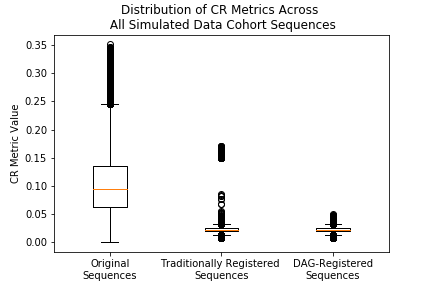
\includegraphics[width=0.5\textwidth]{6/figures/spectr-cr-box.png}
\caption{Boxplots of the values of all correlation ratio matrices for the original sequences, the traditionally registered sequences, and the DAG-registered sequences for the simulated data.}
\label{fig:spectr-cr-box}
\end{figure}

\begin{table}[]
\centering
\caption{Results of t-tests comparing the descriptive statistics of the correlation ratio matrices for the simulated data.}
\label{tab:spectr-cr-ttest}
\begin{tabular}{|c|c|c|c|}
\hline
\textbf{Sequence Type 1 ($S_1$)} &
  \textbf{Original} &
  \textbf{Original} &
  \textbf{\begin{tabular}[c]{@{}c@{}}Traditionally \\ Registered\end{tabular}} \\ \hline
\textbf{Sequence Type 2 ($S_2$)} &
  \textbf{\begin{tabular}[c]{@{}c@{}}Traditionally\\ Registered\end{tabular}} &
  \textbf{\begin{tabular}[c]{@{}c@{}}DAG\\ Registered\end{tabular}} &
  \textbf{\begin{tabular}[c]{@{}c@{}}DAG\\ Registered\end{tabular}} \\ \hline
\begin{tabular}[c]{@{}c@{}}P($S_1$ and $S_2$ \\ have same minimums)\end{tabular} &
  0.3487 &
  0.3407 &
  0.9821 \\ \hline
\begin{tabular}[c]{@{}c@{}}P($S_1$ and $S_2$ \\ have same 1st quartile)\end{tabular} &
  9.750 E -113 &
  1.246 E -112 &
  0.8019 \\ \hline
\begin{tabular}[c]{@{}c@{}}P($S_1$ and $S_2$ \\ have same medians)\end{tabular} &
  5.288 E -88 &
  5.409 E -88 &
  0.9997 \\ \hline
\begin{tabular}[c]{@{}c@{}}P($S_1$ and $S_2$ \\ have same 3rd quartiles)\end{tabular} &
  6.534 E -81 &
  6.730 E -81 &
  0.9577 \\ \hline
\begin{tabular}[c]{@{}c@{}}P($S_1$ and $S_2$ \\ have same maximums)\end{tabular} &
  2.536 E -98 &
  6.180 E -103 &
  0.4068 \\ \hline
\end{tabular}
\end{table}

\begin{figure}
\centering
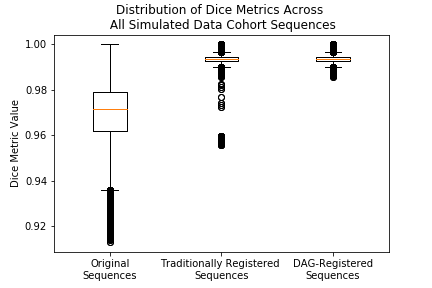
\includegraphics[width=0.5\textwidth]{6/figures/spectr-dice-box.png}
\caption{Boxplots of the values of all Dice matrices for the original sequences, the traditionally registered sequences, and the DAG-registered sequences for the simulated data.}
\label{fig:spectr-dice-box}
\end{figure}

\begin{table}[]
\centering
\caption{Results of t-tests comparing the descriptive statistics of the Dice matrices for the simulated data.}
\label{tab:spectr-dice-ttest}
\begin{tabular}{|c|c|c|c|}
\hline
\textbf{Sequence Type 1 ($S_1$)} &
  \textbf{Original} &
  \textbf{Original} &
  \textbf{\begin{tabular}[c]{@{}c@{}}Traditionally \\ Registered\end{tabular}} \\ \hline
\textbf{Sequence Type 2 ($S_2$)} &
  \textbf{\begin{tabular}[c]{@{}c@{}}Traditionally\\ Registered\end{tabular}} &
  \textbf{\begin{tabular}[c]{@{}c@{}}DAG\\ Registered\end{tabular}} &
  \textbf{\begin{tabular}[c]{@{}c@{}}DAG\\ Registered\end{tabular}} \\ \hline
\begin{tabular}[c]{@{}c@{}}P($S_1$ and $S_2$ \\ have same minimums)\end{tabular} &
  9.976 E -105 &
  2.520 E -110 &
  0.3778 \\ \hline
\begin{tabular}[c]{@{}c@{}}P($S_1$ and $S_2$ \\ have same 1st quartile)\end{tabular} &
  5.225 E -93 &
  5.582 E -93 &
  0.931 \\ \hline
\begin{tabular}[c]{@{}c@{}}P($S_1$ and $S_2$ \\ have same medians)\end{tabular} &
  1.988 E -104 &
  2.158 E -104 &
  0.9578 \\ \hline
\begin{tabular}[c]{@{}c@{}}P($S_1$ and $S_2$ \\ have same 3rd quartiles)\end{tabular} &
  1.679 E -131 &
  2.190 E -131 &
  0.842 \\ \hline
\begin{tabular}[c]{@{}c@{}}P($S_1$ and $S_2$ \\ have same maximums)\end{tabular} &
  1.0 &
  1.0 &
  1.0 \\ \hline
\end{tabular}
\end{table}

\begin{figure}
\centering
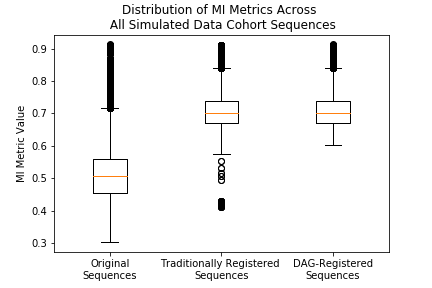
\includegraphics[width=0.5\textwidth]{6/figures/spectr-mi-box.png}
\caption{Boxplots of the values of all mutual information matrices for the original sequences, the traditionally registered sequences, and the DAG-registered sequences for the simulated data.}
\label{fig:spectr-mi-box}
\end{figure}

\begin{table}[]
\centering
\caption{Results of t-tests comparing the descriptive statistics of the MI matrices for the simulated data.}
\label{tab:spectr-mi-ttest}
\begin{tabular}{|c|c|c|c|}
\hline
\textbf{Sequence Type 1 ($S_1$)} &
  \textbf{Original} &
  \textbf{Original} &
  \textbf{\begin{tabular}[c]{@{}c@{}}Traditionally \\ Registered\end{tabular}} \\ \hline
\textbf{Sequence Type 2 ($S_2$)} &
  \textbf{\begin{tabular}[c]{@{}c@{}}Traditionally\\ Registered\end{tabular}} &
  \textbf{\begin{tabular}[c]{@{}c@{}}DAG\\ Registered\end{tabular}} &
  \textbf{\begin{tabular}[c]{@{}c@{}}DAG\\ Registered\end{tabular}} \\ \hline
\begin{tabular}[c]{@{}c@{}}P($S_1$ and $S_2$ \\ have same minimums)\end{tabular} &
  5.016 E -114 &
  6.328 E -126 &
  0.5397 \\ \hline
\begin{tabular}[c]{@{}c@{}}P($S_1$ and $S_2$ \\ have same 1st quartile)\end{tabular} &
  4.68 E -105 &
  7.90 E -105 &
  0.995 \\ \hline
\begin{tabular}[c]{@{}c@{}}P($S_1$ and $S_2$ \\ have same medians)\end{tabular} &
  1.65 E -97 &
  3.57 E -97 &
  0.994 \\ \hline
\begin{tabular}[c]{@{}c@{}}P($S_1$ and $S_2$ \\ have same 3rd quartiles)\end{tabular} &
  1.065 E -84 &
  2.374 E -84 &
  0.974 \\ \hline
\begin{tabular}[c]{@{}c@{}}P($S_1$ and $S_2$ \\ have same maximums)\end{tabular} &
  0.00473 &
  0.00794 &
  0.8761 \\ \hline
\end{tabular}
\end{table}

Motion across the whole sequence was measured by comparing every image volume in the sequence to every other image volume in the sequence. The three metrics used for this comparison were the correlation ratio, the Dice metric, and the mutual information metric. The calculations for a single metric on one sequence produced a two dimensional matrix of metric values. 

These matrices were used to compare the quantities of motion over the course of an entire sequence. For a population level comparison, the minimum, first quartile, median, third quartile, and maximum values of each matrix were computed for each sequence. The distribution of these values for sequences of one sequence type were compared to the distributions for a second sequence type using t-tests. The p-values that each metric comes from a different distribution can be seen in Table \ref{tab:spectr-cr-ttest} for the correlation ratio matrices, Table \ref{tab:spectr-dice-ttest} for the Dice matrices, and Table \ref{tab:spectr-mi-ttest} for the MI matrices. 

More generally, all matrix values for each sequence type were compared using the Kolmogorov-Smirnov test. The distributions for the correlation ratio metrics for the original, the traditionally registered, and the DAG-registered sequences differed at p < 0.005. The distributions for the Dice metrics and the mutual information metrics were also found to be from different distributions for each sequence type at p < 0.005. 

Figures HMM show boxplots of the distributions of each metric over the three sequence types. 

For the first analysis, the metrics matrices were compared to each other 

To compare motion patterns, the metrics matrices were normalized for each subject.


The differences in the motion patterns embodied by the normalized matrices were different between the original, traditionally registered, and DAG-registered sequences for each simulated subject was significant at $p < 0.005$.

Use t-test to compare the normalized matrices for all simulated subjects across a single registration type. Plot a clustermap based on 2 coordinates and the distance (p-value) between them

\subsection{*Volume Registration: Recovered Signal}


\section{Preadolescent Cohort}

\subsection{Volume Registration: Power Thresholds}

\begin{figure}[t]
	\centering
	\begin{subfigure}{0.4\textwidth}
		\centering
		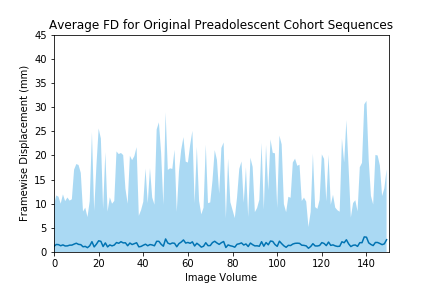
\includegraphics[width=1.0\textwidth]{6/figures/preads-bold-fd-150.png}
		\caption{FD of Original Sequences.}
	\end{subfigure}
	\hspace{0.05\textwidth}
	\begin{subfigure}{0.4\textwidth}
		\centering
		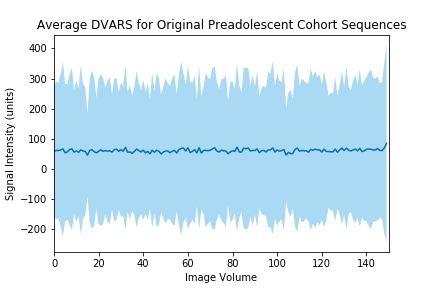
\includegraphics[width=1.0\textwidth]{6/figures/preads-bold-dvars-150.png}
		\caption{DVARS of Original Sequences.}
	\end{subfigure}
	
	\begin{subfigure}{0.4\textwidth}
		\centering
		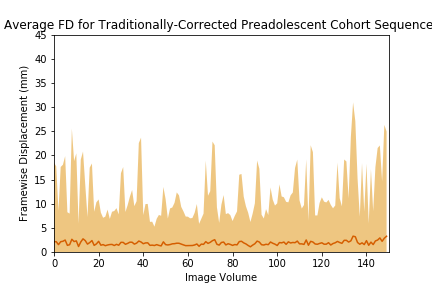
\includegraphics[width=1.0\textwidth]{6/figures/preads-trad-fd-150.png}
		\caption{FD of Traditionally Registered Sequences.}
	\end{subfigure}
	\hspace{0.05\textwidth}
	\begin{subfigure}{0.4\textwidth}
		\centering
		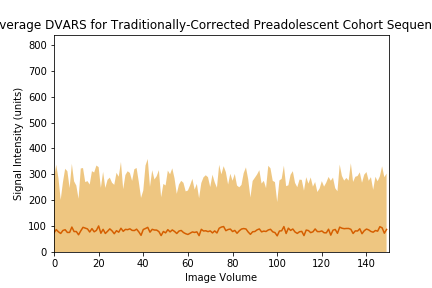
\includegraphics[width=1.0\textwidth]{6/figures/preads-trad-dvars-150.png}
		\caption{DVARS of Traditionally Registered Sequences.}
	\end{subfigure}
	
	\begin{subfigure}{0.4\textwidth}
		\centering
		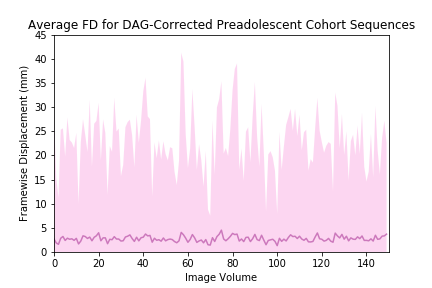
\includegraphics[width=1.0\textwidth]{6/figures/preads-dag-fd-150.png}
		\caption{FD of DAG-Registered Sequences.}
	\end{subfigure}
	\hspace{0.05\textwidth}
	\begin{subfigure}{0.4\textwidth}
		\centering
		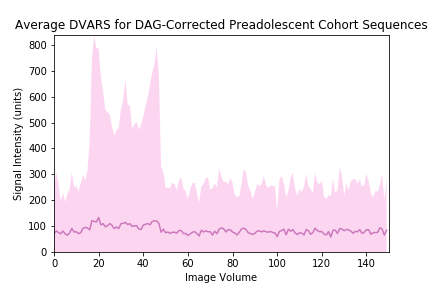
\includegraphics[width=1.0\textwidth]{6/figures/preads-dag-dvars-150.png}
		\caption{DVARS of DAG-Registered Sequences.}
	\end{subfigure}
\caption{The means and standard deviations of the FD and DVARS metrics for all preadolescent images both before and after registration.}
\label{fig:pread-power-dists}
\end{figure}

\begin{table}[h!]
\centering
\caption{The number and percentage of image volumes across all sequences in the preadolescent cohort which meet the usability thresholds of FD \textless 0.2 mm and DVARS \textless 2.5\%.}
\label{tab:pread-power-thresh}
\begin{tabular}{|c|c|c|c|}
\hline
\textbf{Threshold Met} &
  \textbf{\begin{tabular}[c]{@{}c@{}}Original\\  Sequences\end{tabular}} &
  \textbf{\begin{tabular}[c]{@{}c@{}}Traditionally Registered \\ Sequences\end{tabular}} &
  \textbf{\begin{tabular}[c]{@{}c@{}}DAG-Registered \\ Sequences\end{tabular}} \\ \hline
FD (count)    & 107879 & 72104 & 72114 \\ \hline
DVARS (count) & 87169  & 54056 & 53756 \\ \hline
Both (count)  & 74107  & 45006 & 44682 \\ \hline
FD (\%)       & 60.17  & 40.22 & 40.26 \\ \hline
DVARS(\%)     & 48.62  & 30.15 & 30.01 \\ \hline
Both (\%)     & 41.33  & 25.10 & 24.94 \\ \hline
\end{tabular}
\end{table}

Table \ref{tab:pread-power-thresh} contains the number and percentages of image volumes from the whole preadolescent cohort which meet the FD and DVARS thresholds. 

\begin{table}[h!]
\centering
\caption{Results from the t-tests comparing the counts for the numbers of images meeting the FD, DVARS, and FD and DVARS thresholds for sequence type $S_1$ and sequence type $S_2$.}
\label{tab:pread-power-ttest}
\begin{tabular}{|c|c|c|c|}
\hline
\textbf{Sequence Type 1 ($S_1$)} &
  \textbf{Original} &
  \textbf{Original} &
  \textbf{\begin{tabular}[c]{@{}c@{}}Traditionally \\ Registered\end{tabular}} \\ \hline
\textbf{Sequence Type 2 ($S_2$)} &
  \textbf{\begin{tabular}[c]{@{}c@{}}Traditionally\\ Registered\end{tabular}} &
  \textbf{\begin{tabular}[c]{@{}c@{}}DAG\\ Registered\end{tabular}} &
  \textbf{\begin{tabular}[c]{@{}c@{}}DAG\\ Registered\end{tabular}} \\ \hline
\begin{tabular}[c]{@{}c@{}}P($S_1$ and $S_2$ have \\ same FD counts)\end{tabular} &
  2.81 E -16 &
  2.35 E -16 &
  0.998 \\ \hline
\begin{tabular}[c]{@{}c@{}}P($S_1$ and $S_2$ have \\ same DVARS counts)\end{tabular} &
  9.43 E -12 &
  5.30 E -12 &
  0.950 \\ \hline
\begin{tabular}[c]{@{}c@{}}P($S_1$ and $S_2$ have \\ same FD and DVARS counts)\end{tabular} &
  1.12 E -11 &
  5.60 E -12 &
  0.938 \\ \hline
\end{tabular}
\end{table}

Table \ref{tab:pread-power-ttest} shows the results of a set of t-tests which determine if the distribution of metric X for sequence type $S_1$ is the same as the distribution of metric X for sequence type $S_2$.

\begin{table}[h!]
\centering
\caption{The number of subjects whose sequences of types $S_1$ and $S_2$ had different FD distributions.}
\label{tab:pread-fd-kstest}
\begin{tabular}{|c|c|c|c|}
\hline
\textbf{\begin{tabular}[c]{@{}c@{}}\# Sequences \\ Type 1 ($S_1$)\end{tabular}} &
  \textbf{\begin{tabular}[c]{@{}c@{}}\# Sequences \\ Type 2 ($S_2$)\end{tabular}} &
  \textbf{\begin{tabular}[c]{@{}c@{}}\# Sequences \\ p \textless 0.05\end{tabular}} &
  \textbf{\begin{tabular}[c]{@{}c@{}}\# Sequences \\ p \textless 0.005\end{tabular}} \\ \hline
Original                                                            & \begin{tabular}[c]{@{}c@{}}Traditionally\\ Registered\end{tabular} & 331 & 326 \\ \hline
Original                                                            & \begin{tabular}[c]{@{}c@{}}DAG\\ Registered\end{tabular}           & 332 & 328 \\ \hline
\begin{tabular}[c]{@{}c@{}}Traditionally \\ Registered\end{tabular} & \begin{tabular}[c]{@{}c@{}}DAG\\ Registered\end{tabular}           & 19 &17 \\ \hline
\end{tabular}
\end{table}

\begin{table}[h!]
\centering
\caption{The number of subjects whose sequences of types $S_1$ and $S_2$ had different DVARS distributions.}
\label{tab:pread-dvars-kstest}
\begin{tabular}{|c|c|c|c|}
\hline
\textbf{\begin{tabular}[c]{@{}c@{}}\# Sequences \\ Type 1 ($S_1$)\end{tabular}} &
  \textbf{\begin{tabular}[c]{@{}c@{}}\# Sequences \\ Type 2 ($S_2$)\end{tabular}} &
  \textbf{\begin{tabular}[c]{@{}c@{}}\# Sequences \\ p \textless 0.05\end{tabular}} &
  \textbf{\begin{tabular}[c]{@{}c@{}}\# Sequences \\ p \textless 0.005\end{tabular}} \\ \hline
Original                                                            & \begin{tabular}[c]{@{}c@{}}Traditionally\\ Registered\end{tabular} & 334 & 331 \\ \hline
Original                                                            & \begin{tabular}[c]{@{}c@{}}DAG\\ Registered\end{tabular}           & 334 & 333 \\ \hline
\begin{tabular}[c]{@{}c@{}}Traditionally \\ Registered\end{tabular} & \begin{tabular}[c]{@{}c@{}}DAG\\ Registered\end{tabular}           & 22  & 19  \\ \hline
\end{tabular}
\end{table}

% First: FD and DVARs
The averages of the distributions of the FD and DVARs metrics across the whole time period of the sequences for the original, traditionally registered, and DAG-registered images were calculated. The images sequences varied in length from 150 volume to 450 volumes due to the differences in acquisition protocols at different sites. The means and standard deviations of FD and DVARS metrics for the entire set of sequence with their original lengths can be seen in Figures \ref{fig:pread-fd-450} and \ref{fig:pread-dvars-450}. The means and standard deviations of the FD and DVARs metrics for the first 150 volumes in each sequence can be seen in Figures \ref{fig:pread-dvars-150} and \ref{fig:pread-dvars-150}. 


To compare the FD and DVARS values for each type of motion correction, the metrics for each image were considered to be independent samples drawn from an unknown distribution. Pairwise comparisons of these distribution were performed using the Kolmogorov-Smirnov (KS) test. The two-sided KS test measures the distance between the empirical distributions of two distributions. The null hypothesis of the two-sided KS test is that the empirical distributions being compared come from the same underlying distribution. As the KS test is nonparametric, the metrics for all image volumes can be used.

By comparing the distributions for the original sequences to the distributions for the registered sequences, we aim to determine if the volume registration had a significant effect on the images themselves. The comparison of the distributions for the two types of registered images is intended to determine if there is a statistically significant difference between the FD and DVARS distributions of the registered images.


The KS statistic and p-value produced as result of the KS tests can be seen in Table \ref{tab:pread-ks-fd} for the FD metrics and in Table \ref{tab:pread-ks-dvars} for the DVARS metrics.


%Each rs-fMRI sequence in the cohort underwent registration using both frameworks. For each sequence, the correlation ratio between every possible pair of volumes was calculated. A set of metrics of the correlation ratio matrices for each sequence can be seen in Table \ref{tab:crm-stats}. This table shows that the original sequences generally have higher average correlation ratios and contain more variation in their correlation ratios than the globally registered images. The registration methods were able to reduce the mean and variability of the correlation ratios across all subjects in the cohort who had original correlation ratio averages of at least 0.035.



The FD and DVARS values were compared to the usability thresholds defined by Power et al. to determine how many volumes were recovered by each framework \cite{Power2014}. Table \ref{tab:pread-powerthresh} shows the number of volumes meeting each threshold, both in terms of the number of volumes in the cohort and the percentage of volumes in the cohort. In the original dataset, almost 42\% of image volumes met both the FD and DVARS thresholds. However, only about 5\% of volumes met both thresholds for each registration type. Looking at the thresholds independently, about 60\% of volumes met the FD threshold before registration and only 16\% of volumes met the threshold after registration. Similarly, about 48\% of volumes met the DVARS threshold before registration and only about 6\% of volumes met the threshold after registration. These results suggest that the registration process introduces some degree of error into the preadolescent images, at least with respect to the established usability criteria.

\begin{figure}[ht]
\centering
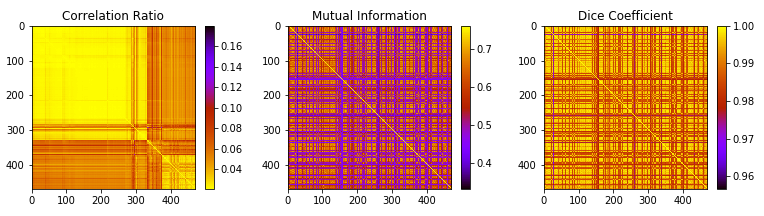
\includegraphics[width=1\textwidth]{6/figures/similarity-mat-sample.png}
\caption{Examples of the three similarity matrices. Lighter colors represent more desirable values.}
\label{fig:sim-mat-sample}
\end{figure}

An example of the three similarity matrices can be seen in Figure \ref{fig:sim-mat-sample}. The element $e_{i,j}$ represents the value of the given metric between the image volumes represented by row $i$ and column $j$. Each metric measures similarity according to slightly different definitions. In this figure, lighter values represent better metric values while darker values indicate lower similarity.

It is important to note the scales for these three metrics vary. The correlation ratio measures the distance between two items. Lower values for the correlation ratio means there is a smaller distance between the given pair of image volumes. The mutual information measures the shared information between two distributions of samples which may or may not be generated from the same underlying distribution. Higher mutual information values mean more shared information and low values mean less shared information. The Dice coefficient measures the overlap of two binary images. High Dice coefficients indicate a large amount of overlap, with a value of 1.0 indicating a perfect overlap.

The correlation ratio matrix in Figure \ref{fig:sim-mat-sample} suggests that the patient remained relatively still for the first 300 volumes of the image, then moved for about 100 volumes, and remained still in a new position for the last 50 frames of the sequence. The colors representing the correlation ratios correspond to very low values, suggesting there is little patient motion overall.

The Dice coefficient matrix has a similar pattern as the mutual information matrix, but leads to a different conclusion. The Dice coefficient was calculated on an Otsu thresholded version of each image volume. As the values of the Dice coefficients are consistently high, the patient likely did not move much. 

The mutual information matrix shows that the shared information throughout the entire image sequence varies. Using the information from the correlation ratio matrix and the Dice coefficient matrix, it is possible that the variations in the mutual information matrix are due to changes in the rs-fMRI signal caused by BOLD signal changes, spin history effects of motion, and susceptibility effects of motion.

\subsection{*Volume Registration: Sequence Duration Motion}

\begin{figure}
\centering
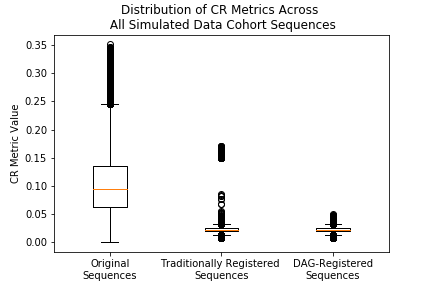
\includegraphics[width=0.5\textwidth]{6/figures/spectr-cr-box.png}
\caption{Boxplots of the values of all correlation ratio matrices for the original sequences, the traditionally registered sequences, and the DAG-registered sequences for the SIMULATED cohort.}
\label{fig:pread-cr-box}
\end{figure}

\begin{table}[]
\centering
\caption{Results of t-tests comparing the descriptive statistics of the correlation ratio matrices for the SIMULATED data.}
\label{tab:pread-cr-ttest}
\begin{tabular}{|c|c|c|c|}
\hline
\textbf{Sequence Type 1 ($S_1$)} &
  \textbf{Original} &
  \textbf{Original} &
  \textbf{\begin{tabular}[c]{@{}c@{}}Traditionally \\ Registered\end{tabular}} \\ \hline
\textbf{Sequence Type 2 ($S_2$)} &
  \textbf{\begin{tabular}[c]{@{}c@{}}Traditionally\\ Registered\end{tabular}} &
  \textbf{\begin{tabular}[c]{@{}c@{}}DAG\\ Registered\end{tabular}} &
  \textbf{\begin{tabular}[c]{@{}c@{}}DAG\\ Registered\end{tabular}} \\ \hline
\begin{tabular}[c]{@{}c@{}}P($S_1$ and $S_2$ \\ have same minimums)\end{tabular} &
  0.3487 &
  0.3407 &
  0.9821 \\ \hline
\begin{tabular}[c]{@{}c@{}}P($S_1$ and $S_2$ \\ have same 1st quartile)\end{tabular} &
  9.750 E -113 &
  1.246 E -112 &
  0.8019 \\ \hline
\begin{tabular}[c]{@{}c@{}}P($S_1$ and $S_2$ \\ have same medians)\end{tabular} &
  5.288 E -88 &
  5.409 E -88 &
  0.9997 \\ \hline
\begin{tabular}[c]{@{}c@{}}P($S_1$ and $S_2$ \\ have same 3rd quartiles)\end{tabular} &
  6.534 E -81 &
  6.730 E -81 &
  0.9577 \\ \hline
\begin{tabular}[c]{@{}c@{}}P($S_1$ and $S_2$ \\ have same maximums)\end{tabular} &
  2.536 E -98 &
  6.180 E -103 &
  0.4068 \\ \hline
\end{tabular}
\end{table}

\begin{figure}
\centering
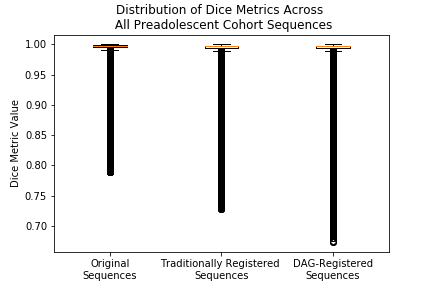
\includegraphics[width=0.5\textwidth]{6/figures/preads-dice-box.png}
\caption{Boxplots of the values of all Dice matrices for the original sequences, the traditionally registered sequences, and the DAG-registered sequences for the preadolescent cohort.}
\label{fig:preads-dice-box}
\end{figure}

\begin{table}[]
\centering
\caption{Results of t-tests comparing the descriptive statistics of the Dice matrices for the preadolescent data.}
\label{tab:preads-dice-ttest}
\begin{tabular}{|c|c|c|c|}
\hline
\textbf{Sequence Type 1 ($S_1$)} &
  \textbf{Original} &
  \textbf{Original} &
  \textbf{\begin{tabular}[c]{@{}c@{}}Traditionally \\ Registered\end{tabular}} \\ \hline
\textbf{Sequence Type 2 ($S_2$)} &
  \textbf{\begin{tabular}[c]{@{}c@{}}Traditionally\\ Registered\end{tabular}} &
  \textbf{\begin{tabular}[c]{@{}c@{}}DAG\\ Registered\end{tabular}} &
  \textbf{\begin{tabular}[c]{@{}c@{}}DAG\\ Registered\end{tabular}} \\ \hline
\begin{tabular}[c]{@{}c@{}}P($S_1$ and $S_2$ \\ have same minimums)\end{tabular} &
  0.770 &
  0.695 &
  0.916 \\ \hline
\begin{tabular}[c]{@{}c@{}}P($S_1$ and $S_2$ \\ have same 1st quartile)\end{tabular} &
  0.976 &
  0.906 &
  0.880 \\ \hline
\begin{tabular}[c]{@{}c@{}}P($S_1$ and $S_2$ \\ have same medians)\end{tabular} &
  0.883 &
  0.562 &
  0.643 \\ \hline
\begin{tabular}[c]{@{}c@{}}P($S_1$ and $S_2$ \\ have same 3rd quartiles)\end{tabular} &
  0.000343 &
  0.000586 &
  0.390 \\ \hline
\begin{tabular}[c]{@{}c@{}}P($S_1$ and $S_2$ \\ have same maximums)\end{tabular} &
  1.0 &
  1.0 &
  1.0 \\ \hline
\end{tabular}
\end{table}

\begin{figure}
\centering
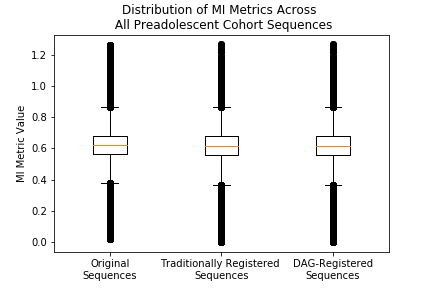
\includegraphics[width=0.5\textwidth]{6/figures/preads-mi-box.png}
\caption{Boxplots of the values of all mutual information matrices for the original sequences, the traditionally registered sequences, and the DAG-registered sequences for the preadolescent cohort.}
\label{fig:preads-mi-box}
\end{figure}

\begin{table}[]
\centering
\caption{Results of t-tests comparing the descriptive statistics of the MI matrices for the preadolescent data.}
\label{tab:preads-mi-ttest}
\begin{tabular}{|c|c|c|c|}
\hline
\textbf{Sequence Type 1 ($S_1$)} &
  \textbf{Original} &
  \textbf{Original} &
  \textbf{\begin{tabular}[c]{@{}c@{}}Traditionally \\ Registered\end{tabular}} \\ \hline
\textbf{Sequence Type 2 ($S_2$)} &
  \textbf{\begin{tabular}[c]{@{}c@{}}Traditionally\\ Registered\end{tabular}} &
  \textbf{\begin{tabular}[c]{@{}c@{}}DAG\\ Registered\end{tabular}} &
  \textbf{\begin{tabular}[c]{@{}c@{}}DAG\\ Registered\end{tabular}} \\ \hline
\begin{tabular}[c]{@{}c@{}}P($S_1$ and $S_2$ \\ have same minimums)\end{tabular} &
  0.624 &
  0.718 &
  0.896 \\ \hline
\begin{tabular}[c]{@{}c@{}}P($S_1$ and $S_2$ \\ have same 1st quartile)\end{tabular} &
  0.489 &
  0.497 &
  0.992 \\ \hline
\begin{tabular}[c]{@{}c@{}}P($S_1$ and $S_2$ \\ have same medians)\end{tabular} &
  0.364 &
  0.324 &
  0.928 \\ \hline
\begin{tabular}[c]{@{}c@{}}P($S_1$ and $S_2$ \\ have same 3rd quartiles)\end{tabular} &
  0.121 &
  0.0882 &
  0.851 \\ \hline
\begin{tabular}[c]{@{}c@{}}P($S_1$ and $S_2$ \\ have same maximums)\end{tabular} &
  0.946 &
  0.932 &
  0.987 \\ \hline
\end{tabular}
\end{table}

The distributions of the metrics matrices were compared to each other using the Kolmogorov-Smirnov test for each sequence type. The metrics for the Dice matrices and the mutual information matrices were determined to be from different distributions for each sequence type at p < 0.005.

%-----------------------------------------------------------------
\section{Neonatal Cohort}

\subsection{Volume Registration: Power Thresholds}

\begin{figure}[t]
	\centering
	\begin{subfigure}{0.4\textwidth}
		\centering
		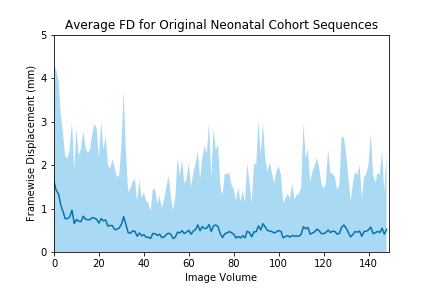
\includegraphics[width=1.0\textwidth]{6/figures/neonates-bold-fd-150.png}
		\caption{FD of Original Sequences.}
	\end{subfigure}
	\hspace{0.05\textwidth}
	\begin{subfigure}{0.4\textwidth}
		\centering
		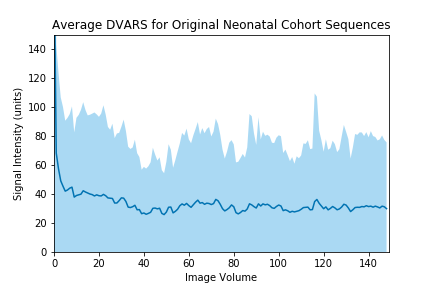
\includegraphics[width=1.0\textwidth]{6/figures/neonates-bold-dvars-150.png}
		\caption{DVARS of Original Sequences.}
	\end{subfigure}
	
	\begin{subfigure}{0.4\textwidth}
		\centering
		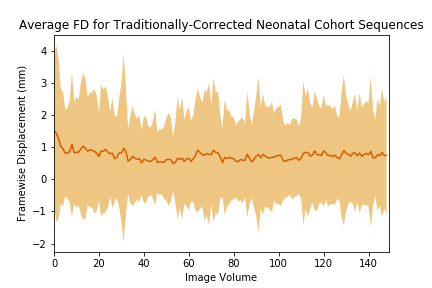
\includegraphics[width=1.0\textwidth]{6/figures/neonates-trad-fd-150.png}
		\caption{FD of Traditionally Registered Sequences.}
	\end{subfigure}
	\hspace{0.05\textwidth}
	\begin{subfigure}{0.4\textwidth}
		\centering
		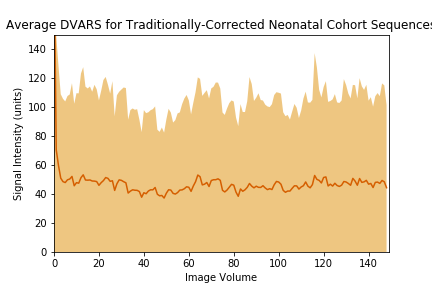
\includegraphics[width=1.0\textwidth]{6/figures/neonates-trad-dvars-150.png}
		\caption{DVARS of Traditionally Registered Sequences.}
	\end{subfigure}
	
	\begin{subfigure}{0.4\textwidth}
		\centering
		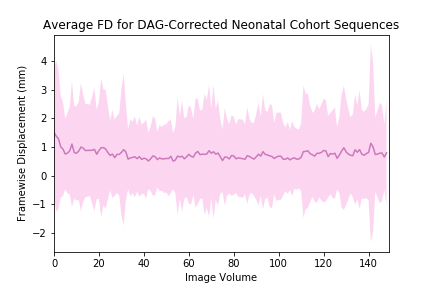
\includegraphics[width=1.0\textwidth]{6/figures/neonates-dag-fd-150.png}
		\caption{FD of DAG-Registered Sequences.}
	\end{subfigure}
	\hspace{0.05\textwidth}
	\begin{subfigure}{0.4\textwidth}
		\centering
		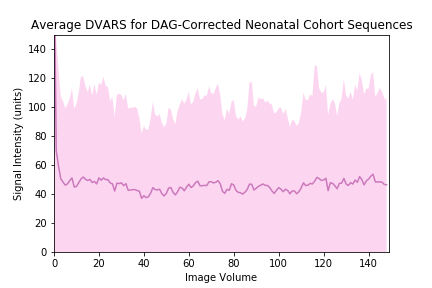
\includegraphics[width=1.0\textwidth]{6/figures/neonates-dag-dvars-150.png}
		\caption{DVARS of DAG-Registered Sequences.}
	\end{subfigure}
\caption{The means and standard deviations of the FD and DVARS metrics for all neonatal images both before and after registration.}
\label{fig:neonate-power-dists}
\end{figure}

\begin{table}[h!]
\centering
\caption{The number and percentage of image volumes across all sequences in the neonatal cohort which meet the usability thresholds of FD \textless 0.2 mm and DVARS \textless 2.5\%.}
\label{tab:neonate-power-thresh}
\begin{tabular}{|c|c|c|c|}
\hline
\textbf{Threshold Met} &
  \textbf{\begin{tabular}[c]{@{}c@{}}Original\\  Sequences\end{tabular}} &
  \textbf{\begin{tabular}[c]{@{}c@{}}Traditionally Registered \\ Sequences\end{tabular}} &
  \textbf{\begin{tabular}[c]{@{}c@{}}DAG-Registered \\ Sequences\end{tabular}} \\ \hline
FD (count)    & 16495  & 14264 & 14173 \\ \hline
DVARS (count) & 16820  & 13903 & 13752 \\ \hline
Both (count)  & 15332  & 12837 & 12684 \\ \hline
FD (\%)       & 69.59  & 60.18 & 59.79 \\ \hline
DVARS(\%)     & 70.96  & 58.65 & 58.02 \\ \hline
Both (\%)     & 64.68  & 54.16 & 53.51 \\ \hline
\end{tabular}
\end{table}

Table \ref{tab:neonate-power-thresh} contains the number and percentages of image volumes from the whole neonatal cohort which meet the FD and DVARS thresholds. The total number of image volumes in across all sequences of a single type was 23704.

\begin{table}[h!]
\centering
\caption{Results from the t-tests comparing the counts for the numbers of images meeting the FD, DVARS, and FD and DVARS thresholds for sequence type $S_1$ and sequence type $S_2$.}
\label{tab:neonate-power-ttest}
\begin{tabular}{|c|c|c|c|}
\hline
\textbf{Sequence Type 1 ($S_1$)} &
  \textbf{Original} &
  \textbf{Original} &
  \textbf{\begin{tabular}[c]{@{}c@{}}Traditionally \\ Registered\end{tabular}} \\ \hline
\textbf{Sequence Type 2 ($S_2$)} &
  \textbf{\begin{tabular}[c]{@{}c@{}}Traditionally\\ Registered\end{tabular}} &
  \textbf{\begin{tabular}[c]{@{}c@{}}DAG\\ Registered\end{tabular}} &
  \textbf{\begin{tabular}[c]{@{}c@{}}DAG\\ Registered\end{tabular}} \\ \hline
\begin{tabular}[c]{@{}c@{}}P($S_1$ and $S_2$ have \\ same FD counts)\end{tabular} &
  0.0110 &
  0.00813 &
  0.924 \\ \hline
\begin{tabular}[c]{@{}c@{}}P($S_1$ and $S_2$ have \\ same DVARS counts)\end{tabular} &
  0.00163 &
  0.000942 &
  0.880 \\ \hline
\begin{tabular}[c]{@{}c@{}}P($S_1$ and $S_2$ have \\ same FD and DVARS counts)\end{tabular} &
  0.00779 &
  0.00475 &
  0.879 \\ \hline
\end{tabular}
\end{table}

Table \ref{tab:neonate-power-ttest} shows the results of a set of t-tests which determine if the distribution of metric X for sequence type $S_1$ is the same as the distribution of metric X for sequence type $S_2$.

\begin{table}[h!]
\centering
\caption{The number of subjects whose sequences of types $S_1$ and $S_2$ had different FD distributions.}
\label{tab:neonate-fd-kstest}
\begin{tabular}{|c|c|c|c|}
\hline
\textbf{\begin{tabular}[c]{@{}c@{}}\# Sequences \\  Type 1 ($S_1$)\end{tabular}} &
  \textbf{\begin{tabular}[c]{@{}c@{}}\# Sequences \\ Type 2 ($S_2$)\end{tabular}} &
  \textbf{\begin{tabular}[c]{@{}c@{}}\# Sequences \\ p \textless 0.05\end{tabular}} &
  \textbf{\begin{tabular}[c]{@{}c@{}}\# Sequences \\ p \textless 0.005\end{tabular}} \\ \hline
Original                                                            & \begin{tabular}[c]{@{}c@{}}Traditionally\\ Registered\end{tabular} & 36	 & 32 \\ \hline
Original                                                            & \begin{tabular}[c]{@{}c@{}}DAG\\ Registered\end{tabular}           & 42 & 38 \\ \hline
\begin{tabular}[c]{@{}c@{}}Traditionally \\ Registered\end{tabular} & \begin{tabular}[c]{@{}c@{}}DAG\\ Registered\end{tabular}           & 13 & 5 \\ \hline
\end{tabular}
\end{table}

\begin{table}[h!]
\centering
\caption{The number of subjects whose sequences of types $S_1$ and $S_2$ had different DVARS distributions.}
\label{tab:neonate-dvars-kstest}
\begin{tabular}{|c|c|c|c|}
\hline
\textbf{\begin{tabular}[c]{@{}c@{}}\# Sequences \\ Type 1($S_1$)\end{tabular}} &
  \textbf{\begin{tabular}[c]{@{}c@{}}\# Sequences \\ Type 2 ($S_2$)\end{tabular}} &
  \textbf{\begin{tabular}[c]{@{}c@{}}\# Sequences \\ p \textless 0.05\end{tabular}} &
  \textbf{\begin{tabular}[c]{@{}c@{}}\# Sequences \\ p \textless 0.005\end{tabular}} \\ \hline
Original                                                            & \begin{tabular}[c]{@{}c@{}}Traditionally\\ Registered\end{tabular} & 44 & 39 \\ \hline
Original                                                            & \begin{tabular}[c]{@{}c@{}}DAG\\ Registered\end{tabular}           & 45 & 44 \\ \hline
\begin{tabular}[c]{@{}c@{}}Traditionally \\ Registered\end{tabular} & \begin{tabular}[c]{@{}c@{}}DAG\\ Registered\end{tabular}           & 11  & 5  \\ \hline
\end{tabular}
\end{table}

\subsection{*Volume Registration: Sequence Duration Motion}

\begin{figure}
\centering
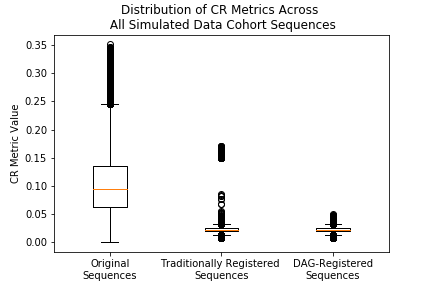
\includegraphics[width=0.5\textwidth]{6/figures/spectr-cr-box.png}
\caption{Boxplots of the values of all correlation ratio matrices for the original sequences, the traditionally registered sequences, and the DAG-registered sequences for the SIMULATED cohort.}
\label{fig:neonates-cr-box}
\end{figure}

\begin{table}[]
\centering
\caption{Results of t-tests comparing the descriptive statistics of the correlation ratio matrices for the SIMULATED data.}
\label{tab:neonates-cr-ttest}
\begin{tabular}{|c|c|c|c|}
\hline
\textbf{Sequence Type 1 ($S_1$)} &
  \textbf{Original} &
  \textbf{Original} &
  \textbf{\begin{tabular}[c]{@{}c@{}}Traditionally \\ Registered\end{tabular}} \\ \hline
\textbf{Sequence Type 2 ($S_2$)} &
  \textbf{\begin{tabular}[c]{@{}c@{}}Traditionally\\ Registered\end{tabular}} &
  \textbf{\begin{tabular}[c]{@{}c@{}}DAG\\ Registered\end{tabular}} &
  \textbf{\begin{tabular}[c]{@{}c@{}}DAG\\ Registered\end{tabular}} \\ \hline
\begin{tabular}[c]{@{}c@{}}P($S_1$ and $S_2$ \\ have same minimums)\end{tabular} &
  0.3487 &
  0.3407 &
  0.9821 \\ \hline
\begin{tabular}[c]{@{}c@{}}P($S_1$ and $S_2$ \\ have same 1st quartile)\end{tabular} &
  9.750 E -113 &
  1.246 E -112 &
  0.8019 \\ \hline
\begin{tabular}[c]{@{}c@{}}P($S_1$ and $S_2$ \\ have same medians)\end{tabular} &
  5.288 E -88 &
  5.409 E -88 &
  0.9997 \\ \hline
\begin{tabular}[c]{@{}c@{}}P($S_1$ and $S_2$ \\ have same 3rd quartiles)\end{tabular} &
  6.534 E -81 &
  6.730 E -81 &
  0.9577 \\ \hline
\begin{tabular}[c]{@{}c@{}}P($S_1$ and $S_2$ \\ have same maximums)\end{tabular} &
  2.536 E -98 &
  6.180 E -103 &
  0.4068 \\ \hline
\end{tabular}
\end{table}

\begin{figure}
\centering
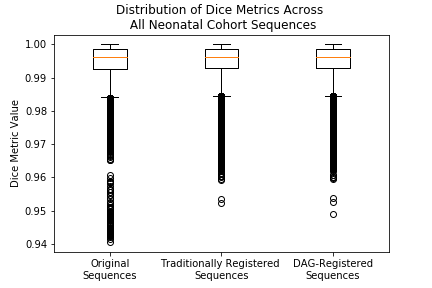
\includegraphics[width=0.5\textwidth]{6/figures/neonates-dice-box.png}
\caption{Boxplots of the values of all Dice matrices for the original sequences, the traditionally registered sequences, and the DAG-registered sequences for the neonatal cohort.}
\label{fig:neonates-dice-box}
\end{figure}

\begin{table}[]
\centering
\caption{Results of t-tests comparing the descriptive statistics of the Dice matrices for the neonatal cohort.}
\label{tab:neonates-dice-ttest}
\begin{tabular}{|c|c|c|c|}
\hline
\textbf{Sequence Type 1 ($S_1$)} &
  \textbf{Original} &
  \textbf{Original} &
  \textbf{\begin{tabular}[c]{@{}c@{}}Traditionally \\ Registered\end{tabular}} \\ \hline
\textbf{Sequence Type 2 ($S_2$)} &
  \textbf{\begin{tabular}[c]{@{}c@{}}Traditionally\\ Registered\end{tabular}} &
  \textbf{\begin{tabular}[c]{@{}c@{}}DAG\\ Registered\end{tabular}} &
  \textbf{\begin{tabular}[c]{@{}c@{}}DAG\\ Registered\end{tabular}} \\ \hline
\begin{tabular}[c]{@{}c@{}}P($S_1$ and $S_2$ \\ have same minimums)\end{tabular} &
  0.523 &
  0.542 &
  0.977 \\ \hline
\begin{tabular}[c]{@{}c@{}}P($S_1$ and $S_2$ \\ have same 1st quartile)\end{tabular} &
  0.468 &
  0.515 &
  0.933 \\ \hline
\begin{tabular}[c]{@{}c@{}}P($S_1$ and $S_2$ \\ have same medians)\end{tabular} &
  0.329 &
  0.292 &
  0.937 \\ \hline
\begin{tabular}[c]{@{}c@{}}P($S_1$ and $S_2$ \\ have same 3rd quartiles)\end{tabular} &
  0.149 &
  0.115 &
  0.890 \\ \hline
\begin{tabular}[c]{@{}c@{}}P($S_1$ and $S_2$ \\ have same maximums)\end{tabular} &
  1.0 &
  1.0 &
  1.0 \\ \hline
\end{tabular}
\end{table}

\begin{figure}
\centering
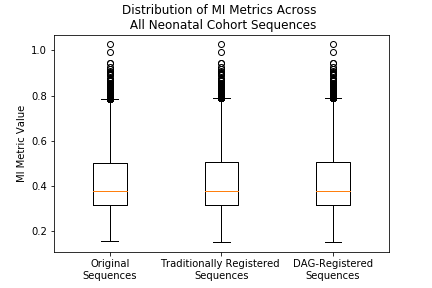
\includegraphics[width=0.5\textwidth]{6/figures/neonates-mi-box.png}
\caption{Boxplots of the values of all mutual information matrices for the original sequences, the traditionally registered sequences, and the DAG-registered sequences for the neonatal cohort.}
\label{fig:neonates-mi-box}
\end{figure}

\begin{table}[]
\centering
\caption{Results of t-tests comparing the descriptive statistics of the MI matrices for the neonatal data.}
\label{tab:neonates-mi-ttest}
\begin{tabular}{|c|c|c|c|}
\hline
\textbf{Sequence Type 1 ($S_1$)} &
  \textbf{Original} &
  \textbf{Original} &
  \textbf{\begin{tabular}[c]{@{}c@{}}Traditionally \\ Registered\end{tabular}} \\ \hline
\textbf{Sequence Type 2 ($S_2$)} &
  \textbf{\begin{tabular}[c]{@{}c@{}}Traditionally\\ Registered\end{tabular}} &
  \textbf{\begin{tabular}[c]{@{}c@{}}DAG\\ Registered\end{tabular}} &
  \textbf{\begin{tabular}[c]{@{}c@{}}DAG\\ Registered\end{tabular}} \\ \hline
\begin{tabular}[c]{@{}c@{}}P($S_1$ and $S_2$ \\ have same minimums)\end{tabular} &
  0.853 &
  0.874 &
  0.978 \\ \hline
\begin{tabular}[c]{@{}c@{}}P($S_1$ and $S_2$ \\ have same 1st quartile)\end{tabular} &
  0.794 &
  0.809 &
  0.985 \\ \hline
\begin{tabular}[c]{@{}c@{}}P($S_1$ and $S_2$ \\ have same medians)\end{tabular} &
  0.762 &
  0.758 &
  0.996 \\ \hline
\begin{tabular}[c]{@{}c@{}}P($S_1$ and $S_2$ \\ have same 3rd quartiles)\end{tabular} &
  0.755 &
  0.743 &
  0.987 \\ \hline
\begin{tabular}[c]{@{}c@{}}P($S_1$ and $S_2$ \\ have same maximums)\end{tabular} &
  0.956 &
  0.938 &
  0.982 \\ \hline
\end{tabular}
\end{table}

The distributions of the metrics matrices were compared to each other using the Kolmogorov-Smirnov test for each sequence type. The metrics for the Dice matrices and the mutual information matrices were determined to be from different distributions for each sequence type at p < 0.005.

\section{*Fetal Cohort}

\subsection{Brain}

\subsubsection{Volume Registration: Power Thresholds}


\begin{figure}[t]
	\centering
	\begin{subfigure}{0.4\textwidth}
		\centering
		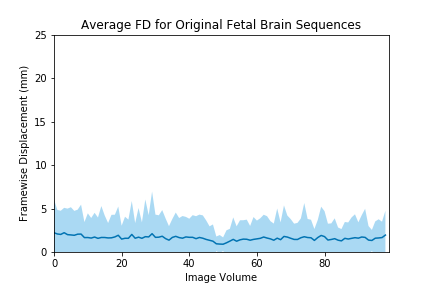
\includegraphics[width=1.0\textwidth]{6/figures/fetal-brain-bold-fd-150.png}
		\caption{FD of Original Sequences.}
	\end{subfigure}
	\hspace{0.05\textwidth}
	\begin{subfigure}{0.4\textwidth}
		\centering
		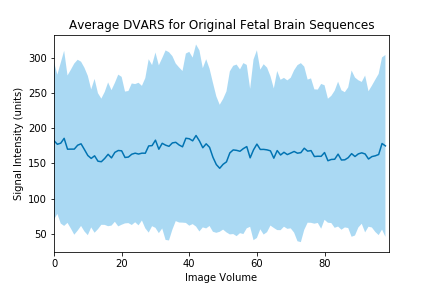
\includegraphics[width=1.0\textwidth]{6/figures/fetal-brain-bold-dvars-150.png}
		\caption{DVARS of Original Sequences.}
	\end{subfigure}
	
	\begin{subfigure}{0.4\textwidth}
		\centering
		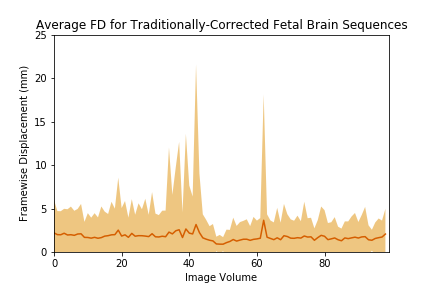
\includegraphics[width=1.0\textwidth]{6/figures/fetal-brain-trad-fd-150.png}
		\caption{FD of Traditionally Registered Sequences.}
	\end{subfigure}
	\hspace{0.05\textwidth}
	\begin{subfigure}{0.4\textwidth}
		\centering
		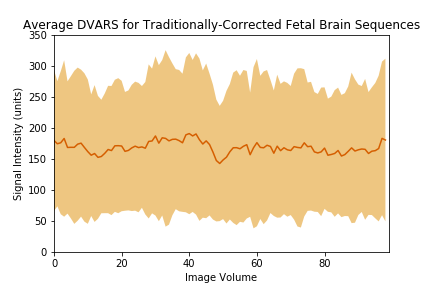
\includegraphics[width=1.0\textwidth]{6/figures/fetal-brain-trad-dvars-150.png}
		\caption{DVARS of Traditionally Registered Sequences.}
	\end{subfigure}
	
	\begin{subfigure}{0.4\textwidth}
		\centering
		\includegraphics[width=1.0\textwidth]{6/figures/fetal-brain-dag-fd-150.png}
		\caption{FD of DAG-Registered Sequences.}
	\end{subfigure}
	\hspace{0.05\textwidth}
	\begin{subfigure}{0.4\textwidth}
		\centering
		\includegraphics[width=1.0\textwidth]{6/figures/fetal-brain-dag-dvars-150.png}
		\caption{DVARS of DAG-Registered Sequences.}
	\end{subfigure}
\caption{The means and standard deviations of the FD and DVARS metrics for all fetal brain images both before and after registration.}
\label{fig:fetal-brain-power-dists}
\end{figure}

\begin{table}[h!]
\centering
\caption{The number and percentage of image volumes across all sequences in the fetal brain image data set which meet the usability thresholds of FD \textless 0.2 mm and DVARS \textless 2.5\%.}
\label{tab:fetal-brain-power-thresh}
\begin{tabular}{|c|c|c|c|}
\hline
\textbf{Threshold Met} &
  \textbf{\begin{tabular}[c]{@{}c@{}}Original\\  Sequences\end{tabular}} &
  \textbf{\begin{tabular}[c]{@{}c@{}}Traditionally Registered \\ Sequences\end{tabular}} &
  \textbf{\begin{tabular}[c]{@{}c@{}}DAG-Registered \\ Sequences\end{tabular}} \\ \hline
FD (count)    & 575    & 539   & 561 \\ \hline
DVARS (count) & 7      & 84    & 7 \\ \hline
Both (count)  & 7      & 80    & 7 \\ \hline
FD (\%)       & 4.775  & 4.503 & 4.659 \\ \hline
DVARS(\%)     & 0.058  & 0.702 & 0.058 \\ \hline
Both (\%)     & 0.058  & 0.668 & 0.058 \\ \hline
\end{tabular}
\end{table}

Table \ref{tab:fetal-brain-power-thresh} contains the number and percentages of image volumes from the whole neonatal cohort which meet the FD and DVARS thresholds. The total number of image volumes in across all sequences of a single type was 12041.

\begin{table}[h!]
\centering
\caption{Results from the t-tests comparing the counts for the numbers of images meeting the FD, DVARS, and FD and DVARS thresholds for fetal brain sequence type $S_1$ and sequence type $S_2$.}
\label{tab:fetal-brain-power-ttest}
\begin{tabular}{|c|c|c|c|}
\hline
\textbf{Sequence Type 1 ($S_1$)} &
  \textbf{Original} &
  \textbf{Original} &
  \textbf{\begin{tabular}[c]{@{}c@{}}Traditionally \\ Registered\end{tabular}} \\ \hline
\textbf{Sequence Type 2 ($S_2$)} &
  \textbf{\begin{tabular}[c]{@{}c@{}}Traditionally\\ Registered\end{tabular}} &
  \textbf{\begin{tabular}[c]{@{}c@{}}DAG\\ Registered\end{tabular}} &
  \textbf{\begin{tabular}[c]{@{}c@{}}DAG\\ Registered\end{tabular}} \\ \hline
\begin{tabular}[c]{@{}c@{}}P($S_1$ and $S_2$ have \\ same FD counts)\end{tabular} &
  0.811 &
  0.926 &
  0.883 \\ \hline
\begin{tabular}[c]{@{}c@{}}P($S_1$ and $S_2$ have \\ same DVARS counts)\end{tabular} &
  0.159 &
  1.0 &
  0.159 \\ \hline
\begin{tabular}[c]{@{}c@{}}P($S_1$ and $S_2$ have \\ same FD and DVARS counts)\end{tabular} &
  0.159 &
  1.0 &
  0.159 \\ \hline
\end{tabular}
\end{table}

Table \ref{tab:fetal-brain-power-ttest} shows the results of a set of t-tests which determine if the distribution of metric X for sequence type $S_1$ is the same as the distribution of metric X for sequence type $S_2$. Fetal brain.

\begin{table}[h!]
\centering
\caption{The number of subjects whose sequences of types $S_1$ and $S_2$ had different FD distributions according to the Kolmogorov-Smirnov test.}
\label{tab:fetal-brain-fd-kstest}
\begin{tabular}{|c|c|c|c|}
\hline
\textbf{\begin{tabular}[c]{@{}c@{}}\# Sequences \\ Type 1 ($S_1$)\end{tabular}} &
  \textbf{\begin{tabular}[c]{@{}c@{}}\# Sequences \\ Type 2 ($S_2$)\end{tabular}} &
  \textbf{\begin{tabular}[c]{@{}c@{}}\# Sequences \\ p \textless 0.05\end{tabular}} &
  \textbf{\begin{tabular}[c]{@{}c@{}}\# Sequences \\ p \textless 0.005\end{tabular}} \\ \hline
Original                                                            & \begin{tabular}[c]{@{}c@{}}Traditionally\\ Registered\end{tabular} & 14 & 9 \\ \hline
Original                                                            & \begin{tabular}[c]{@{}c@{}}DAG\\ Registered\end{tabular}           & 2  & 2 \\ \hline
\begin{tabular}[c]{@{}c@{}}Traditionally \\ Registered\end{tabular} & \begin{tabular}[c]{@{}c@{}}DAG\\ Registered\end{tabular}           & 13 & 9 \\ \hline
\end{tabular}
\end{table}

\begin{table}[h!]
\centering
\caption{The number of subjects whose sequences of types $S_1$ and $S_2$ had different DVARS distributions according to the Kolmogorov-Smirnov test.}
\label{tab:fetal-brain-dvars-kstest}
\begin{tabular}{|c|c|c|c|}
\hline
\textbf{\begin{tabular}[c]{@{}c@{}}\# Sequences \\ Type 1 ($S_1$)\end{tabular}} &
  \textbf{\begin{tabular}[c]{@{}c@{}}\# Sequences \\ Type 2 ($S_2$)\end{tabular}} &
  \textbf{\begin{tabular}[c]{@{}c@{}}\# Sequences \\ p \textless 0.05\end{tabular}} &
  \textbf{\begin{tabular}[c]{@{}c@{}}\# Sequences \\ p \textless 0.005\end{tabular}} \\ \hline
Original                                                            & \begin{tabular}[c]{@{}c@{}}Traditionally\\ Registered\end{tabular} & 3 & 3 \\ \hline
Original                                                            & \begin{tabular}[c]{@{}c@{}}DAG\\ Registered\end{tabular}           & 2 & 1 \\ \hline
\begin{tabular}[c]{@{}c@{}}Traditionally \\ Registered\end{tabular} & \begin{tabular}[c]{@{}c@{}}DAG\\ Registered\end{tabular}           & 2  & 2  \\ \hline
\end{tabular}
\end{table}

\begin{table}[h!]
\centering
\caption{Comparing the FD and DVARS distributions for all image volumes for sequence types $S_1$ and $S_2$ for the fetal brain images.}
\label{tab:fetal-brain-ks-all}
\begin{tabular}{|c|c|c|c|}
\hline
\textbf{Sequence Type 1} & \textbf{Sequence Type 2}                                           & \textbf{FD p-value} & \textbf{DVARS p-value} \\ \hline
Original                 & \begin{tabular}[c]{@{}c@{}}Traditionally\\ Registered\end{tabular} & 2.712 E -10         & 8.019 E -6             \\ \hline
Original                 & \begin{tabular}[c]{@{}c@{}}DAG\\ Registered\end{tabular}           & 0.703               & 0.934                  \\ \hline
\begin{tabular}[c]{@{}c@{}}Traditionally \\ Registered\end{tabular} & \begin{tabular}[c]{@{}c@{}}DAG\\ Registered\end{tabular} & 4.88 E -8 & 0.000380 \\ \hline
\end{tabular}
\end{table}

\subsubsection{Volume Registration: Sequence Duration Motion}

\subsection{Placenta}

\subsubsection{Volume Registration: Power Thresholds}


\begin{table}[h!]
\centering
\caption{The number and percentage of image volumes across all sequences in the fetal placenta image data set which meet the usability thresholds of FD \textless 0.2 mm and DVARS \textless 2.5\%.}
\label{tab:fetal-placenta-power-thresh}
\begin{tabular}{|c|c|c|c|}
\hline
\textbf{Threshold Met} &
  \textbf{\begin{tabular}[c]{@{}c@{}}Original\\  Sequences\end{tabular}} &
  \textbf{\begin{tabular}[c]{@{}c@{}}Traditionally Registered \\ Sequences\end{tabular}} &
  \textbf{\begin{tabular}[c]{@{}c@{}}DAG-Registered \\ Sequences\end{tabular}} \\ \hline
FD (count)    & 575    & 539   & 561 \\ \hline
DVARS (count) & 7      & 84    & 7 \\ \hline
Both (count)  & 7      & 80    & 7 \\ \hline
FD (\%)       & 4.775  & 4.503 & 4.659 \\ \hline
DVARS(\%)     & 0.058  & 0.702 & 0.058 \\ \hline
Both (\%)     & 0.058  & 0.668 & 0.058 \\ \hline
\end{tabular}
\end{table}

Table \ref{tab:fetal-brain-power-thresh} contains the number and percentages of image volumes from the whole neonatal cohort which meet the FD and DVARS thresholds. The total number of image volumes in across all sequences of a single type was 12041.

\begin{table}[h!]
\centering
\caption{Results from the t-tests comparing the counts for the numbers of images meeting the FD, DVARS, and FD and DVARS thresholds for fetal brain sequence type $S_1$ and sequence type $S_2$.}
\label{tab:fetal-brain-power-ttest}
\begin{tabular}{|c|c|c|c|}
\hline
\textbf{Sequence Type 1 ($S_1$)} &
  \textbf{Original} &
  \textbf{Original} &
  \textbf{\begin{tabular}[c]{@{}c@{}}Traditionally \\ Registered\end{tabular}} \\ \hline
\textbf{Sequence Type 2 ($S_2$)} &
  \textbf{\begin{tabular}[c]{@{}c@{}}Traditionally\\ Registered\end{tabular}} &
  \textbf{\begin{tabular}[c]{@{}c@{}}DAG\\ Registered\end{tabular}} &
  \textbf{\begin{tabular}[c]{@{}c@{}}DAG\\ Registered\end{tabular}} \\ \hline
\begin{tabular}[c]{@{}c@{}}P($S_1$ and $S_2$ have \\ same FD counts)\end{tabular} &
  0.811 &
  0.926 &
  0.883 \\ \hline
\begin{tabular}[c]{@{}c@{}}P($S_1$ and $S_2$ have \\ same DVARS counts)\end{tabular} &
  0.159 &
  1.0 &
  0.159 \\ \hline
\begin{tabular}[c]{@{}c@{}}P($S_1$ and $S_2$ have \\ same FD and DVARS counts)\end{tabular} &
  0.159 &
  1.0 &
  0.159 \\ \hline
\end{tabular}
\end{table}

Table \ref{tab:fetal-brain-power-ttest} shows the results of a set of t-tests which determine if the distribution of metric X for sequence type $S_1$ is the same as the distribution of metric X for sequence type $S_2$. Fetal brain.

\begin{table}[h!]
\centering
\caption{The number of subjects whose sequences of types $S_1$ and $S_2$ had different FD distributions according to the Kolmogorov-Smirnov test.}
\label{tab:fetal-brain-fd-kstest}
\begin{tabular}{|c|c|c|c|}
\hline
\textbf{\begin{tabular}[c]{@{}c@{}}\# Sequences \\ Type 1 ($S_1$)\end{tabular}} &
  \textbf{\begin{tabular}[c]{@{}c@{}}\# Sequences \\ Type 2 ($S_2$)\end{tabular}} &
  \textbf{\begin{tabular}[c]{@{}c@{}}\# Sequences \\ p \textless 0.05\end{tabular}} &
  \textbf{\begin{tabular}[c]{@{}c@{}}\# Sequences \\ p \textless 0.005\end{tabular}} \\ \hline
Original                                                            & \begin{tabular}[c]{@{}c@{}}Traditionally\\ Registered\end{tabular} & 14 & 9 \\ \hline
Original                                                            & \begin{tabular}[c]{@{}c@{}}DAG\\ Registered\end{tabular}           & 2  & 2 \\ \hline
\begin{tabular}[c]{@{}c@{}}Traditionally \\ Registered\end{tabular} & \begin{tabular}[c]{@{}c@{}}DAG\\ Registered\end{tabular}           & 13 & 9 \\ \hline
\end{tabular}
\end{table}

\begin{table}[h!]
\centering
\caption{The number of subjects whose sequences of types $S_1$ and $S_2$ had different DVARS distributions according to the Kolmogorov-Smirnov test.}
\label{tab:fetal-brain-dvars-kstest}
\begin{tabular}{|c|c|c|c|}
\hline
\textbf{\begin{tabular}[c]{@{}c@{}}\# Sequences \\ Type 1 ($S_1$)\end{tabular}} &
  \textbf{\begin{tabular}[c]{@{}c@{}}\# Sequences \\ Type 2 ($S_2$)\end{tabular}} &
  \textbf{\begin{tabular}[c]{@{}c@{}}\# Sequences \\ p \textless 0.05\end{tabular}} &
  \textbf{\begin{tabular}[c]{@{}c@{}}\# Sequences \\ p \textless 0.005\end{tabular}} \\ \hline
Original                                                            & \begin{tabular}[c]{@{}c@{}}Traditionally\\ Registered\end{tabular} & 3 & 3 \\ \hline
Original                                                            & \begin{tabular}[c]{@{}c@{}}DAG\\ Registered\end{tabular}           & 2 & 1 \\ \hline
\begin{tabular}[c]{@{}c@{}}Traditionally \\ Registered\end{tabular} & \begin{tabular}[c]{@{}c@{}}DAG\\ Registered\end{tabular}           & 2  & 2  \\ \hline
\end{tabular}
\end{table}

\begin{table}[h!]
\centering
\caption{Comparing the FD and DVARS distributions for all image volumes for sequence types $S_1$ and $S_2$ for the fetal brain images.}
\label{tab:fetal-brain-ks-all}
\begin{tabular}{|c|c|c|c|}
\hline
\textbf{Sequence Type 1} & \textbf{Sequence Type 2}                                           & \textbf{FD p-value} & \textbf{DVARS p-value} \\ \hline
Original                 & \begin{tabular}[c]{@{}c@{}}Traditionally\\ Registered\end{tabular} & 2.712 E -10         & 8.019 E -6             \\ \hline
Original                 & \begin{tabular}[c]{@{}c@{}}DAG\\ Registered\end{tabular}           & 0.703               & 0.934                  \\ \hline
\begin{tabular}[c]{@{}c@{}}Traditionally \\ Registered\end{tabular} & \begin{tabular}[c]{@{}c@{}}DAG\\ Registered\end{tabular} & 4.88 E -8 & 0.000380 \\ \hline
\end{tabular}
\end{table}

\subsubsection{Volume Registration: Sequence Duration Motion}

\section{Motion Patterns}

\subsection{Age Groups}

\subsection{CHD and Control}

\subsection{Preadolescents: Comparing Sites}

%\chapter{DISCUSSION}
\label{ch:discussion}

\section{Volume Registration}

The comparison of the simulated and clinical brain rs-fMRIs using the FD and DVARS metrics showed little difference with respect to reducing the positional and signal effects of motion between pairs of subsequent time points. In the set of placenta images, both registration types improved the number of image volumes meeting the DVARS thresholds. These metrics were not considered sufficient for examining the effects of registration on patient motion, so the similarity matrices were employed. For the simulated data cohort, the minimum values and quartiles of the distributions of the Dice and MI matrices increased more for the DAG-registered sequences than for the original sequences. The changes in the similarity matrix distributions was comparable overall for the clinical images.

An additional analysis was performed for the simulated images. The goal of this analysis was to evaluate the effects of volume registration on the brain signal present in an rs-fMRI image. It was found that the DAG-registered sequences had correct voxel classifications when compared to the DMN ROI than the traditional registration did. 

This finding has interesting potential. Subject motion during rs-MRI scans affects both the recorded position and orientation of the subject as well as the established magnetic spin gradients within the skull and the susecptibility recorded in each voxel. The primary focus of volume registration has been to reduce the positional effects of motion. Correction of the spin history effects and the susceptibility effects are considered to be a separate albeit related area of research. The results of the independent component analysis of the simulated images suggest that the DAG-based registration may contribute to the reduction of the signal-based effects of motion. It could potentially be coupled with prospective motion monitoring techniques, $B_0$ field maps, and navigator sequences to address the other half of the motion problem.

All images used in these analyses consisted of brain tissue against an empty background. The images had undergone processing to remove tissues outside the skull either using automated tools or manual segmentation. The use of manual segmentation with multiple annotators has the potential to confound the results of motion correction experiments. The segmentation process may not remove all non-brain tissue from the image. Those images would then contain brain tissue, non-brain tissue, and dark background. The registration process optimizes the alignment of values in a pair of images. In some cases, the registration reach a state where the lowest cost alignment aligns tissue in general and not specifically brain tissue. While these alignments would have the lowest cost, the would not be physically correct. This problem would be difficult to detect in the metrics extracted from the image sequence: the metrics only measure the properties of the voxel values in the sequence, not of the physiological information it contains. 

Specifically, this limitation pertains to our fetal scans. The masks generated during the segmentation process were created to be uniform across the whole sequence. However, fetal motion is highly variable. The subject may drastically change position in the middle of the scan, possibly several times. The manually created masks were developed using a software tool which allows 3D image masks to be applied to an entire 4D image sequence. The masks were required to be created to ensure the fetal brain or placenta would be inside the masked area at all times and therefore may not have removed all tissues that were not of interest.

This limitation can be resolved by incorporating computer vision principles into the anatomical aspects of image segmentation. Filters used in computer vision applications to identify edges, smooth areas, and track objects have great potential when applied to segmenting fetal brain tissue in the presence of motion.

\section{Characterizing Motion}

In addition to the evaluation of motion within the images, clustering techniques were used to identify groups of subjects with similar motion patterns in their original sequences. Agglomerative clustering was used to confirm the existence of similar motion patterns between patients. The agglomerative clustering results consisting of a heatmap and a dendrogram were combined with two sets of labels: the disease status and age group of each subject. Examination of the dendrograms and heatmaps coupled with the labels suggested that subjects in the same age group were more likely to exhibit similar motion patterns to each other than to subjects in other age groups. To reinforce this theory, k-means clustering and spectral clustering were also performed on the data. The labels produced by the clustering techniques were compared to the age group labels. The composition of the clusters reinforces the theory that patient motion patterns vary more between age groups than among age groups.

Additional analyses could be performed to further evaluate the computer detectable differences in patient groups. The models presented in the previous chapter were generated each using a single metric type. Each metric only measures one property of the image volumes. It is possible that combinations of metrics measuring different properties could be used to better separate patient groups. For example, the combination of the FD values and the DVARS values could more comprehensively categorize subjects based on the effects of motion, BOLD signal change, and background noise.

\section{Relation to Existing Work}

\subsection{MRI Simulations} 

The idea of simulated MRIs originated in the 1980s. Bobman et al. suggested a process of MR image synthesis, then demonstrated its validity by creating synthetic spin-echo brain MRIs and comparing the simulated images to clinical images \cite{Bobman1985}. Since then, a number of MRI simulation softwares have been developed. Herein, we discuss two of these tools and compare them to our simulation tool.

The FMRIB group developed a simulation tool called \href{https://fsl.fmrib.ox.ac.uk/fsl/fslwiki/POSSUM}{POSSUM} (Physics-Oriented Simulated Scanner for Understanding MRI) \cite{Drobnjak2006} \cite{Drobnjak2010}. POSSUM offers realistic, physics-based simulation of structural, functional, and diffusion tensor images. It requires a gradient echo pulse sequence and a segmented object with known tissue properties as inputs for the simulation. It allows the user a high degree of control over the physical properties to be simulated. The user has the ability to specify the pulse sequence information, the method for generating brain signal, the addition of motion and noise, and the method for image reconstruction. Both a GUI and a command line interface are available for POSSUM. 

\begin{figure}
\centering
\includegraphics[width=.6\textwidth]{7/possum-gui.png}
\caption{The ``Pulse Sequence'' specifications page in the POSSUM GUI}
\label{fig:possum}
\end{figure}

The biggest drawback to POSSUM is the degree of MR physics knowledge needed to use it effectively. For MR physicists, specifying the details of a pulse sequence may be trivial. For researchers from other fields, customizing pulse sequence parameters, an example of which can be seen in Figure \ref{fig:possum}, can be a challenging task. These customizations may even be unnecessary depending on the goals a researcher hopes to achieve using the simulated data.

If a researcher's goal is to test the impact of a new MRI processing technique on known signals in an image, the BrainWeb MRI simulator might be a better option than POSSUM. BrainWeb was created and is actively developed by the \href{mcgill.ca/bic/}{McConnell Brain Imaging Centre} at McGill University to assist in validation computer-aided MRI analysis tools \cite{kwan1999mri} \cite{collins1998design} \cite{cocosco1997brainweb} \cite{kwan1996extensible}. A set of simulated images have been generated using BrainWeb and are can be found in the BrainWeb Simulated Brain Database (SBD). The SBD contains simulated images for healthy subjects and for subjects who have lesions due to multiple sclerosis.

Custom simulations can be generated on the BrainWeb server by submitting a request via a browser. The simulation request form has three areas which can be customized: the type of brain to simulate, the MR pulse sequence, and the imaging artifacts. The simulation is run on the server and the user is notified via email when the simulated images are ready to download. 

BrainWeb's simulator is slightly more approachable than POSSUM: a limited number of pulse sequence parameters are available to customize and a description is listed next to each parameter in the pulse sequence and imaging artifacts sections. However, the user has slightly less control over the simulated image. The brain models used by BrainWeb are healthy brains or brains with MS lesions. It is not an option for the user to upload an image to use as the structural information in the sequence. For our purposes, the biggest limitation of BrainWeb is that it only simulates structural images. 

Our simulation tool, SPECTr, is one of the few tools which simulates resting-state fMRIs. It offers the opportunity for researchers to explore the effects of their motion correction techniques on BOLD signal, background noise, and patient motion using a lightweight simulation that can be run on a personal computer. It should be noted that SPECTr is not a substitute for the physics-based models in POSSUM and BrainWeb: it is intended to evaluate signal changes in rs-fMRI sequences as a result of post-acquisition image processing.

\subsection{Volume Registration} 

To the best of our knowledge, the only other study that has used a variant of the DAG-based method was performed by Liao et al \cite{Liao2016}. Liao et al’s dataset consisted of 10 fetal rs-fMRIs. In each of these sequences, the fetal brain, fetal liver, and placenta were manually segmented in the first volume of the sequence as well as in five other randomly chosen volumes. These overlap of these manual segmentations before and after registration as measured using the Dice coefficient was used to quantify the amount of motion in each sequence. Even though the Dice coefficients increase more in each sequence after Liao et al.’s registration than after traditional registration, their measure of positional change fails to quantify any changes in position between any other pairs of volumes that do not have manual segmentations. 

The fetal images used in Liao et al.'s study included images of singleton, twin, and triplet pregnancies. There is significant potential value in the study of fetal motion in multifetal pregnancies. Considering the motion patterns alone, it would be expected that the singleton pregnancies have different motion patterns than the multifetal pregnancies

\subsection{Age Group Specific Motion}

It has been established that motion is often correlated with patient age in adolescent population. Satterthwaite et al. specifically designed an imaging study of adolescents ages 8-23 such that patient age and motion were uncorrelated \cite{Satterthwaite2012} % ELEPHANTS check citation
In our study, patient age was described only as fetal, neonatal, or preadolescent despite a range of ages in each group. We establish that there are characteristics of patient motion specific to each group, but we did not consider more granular ranges of patient age. Additional analyses would need to be considered to determine whether post-conceptual age for fetal and neonatal subjects impacts motion characteristics. 

In the fetal cohort, it is possible that there are motion characteristics linked to post-conceptual age. As a fetus grows, the amount of room in the uterus in which it can move decreases. However, as the fetal brain develops, the fetus may begin to move in different ways to test its biological systems. 

Studies involving neonatal cohorts often track two ages for the subjects: the post-conceptual age and the age since birth. The relationship between these two ages and a neonate's brain development could impact the amount of motion exhibited during a scan.
%\chapter{Conclusions}
This is the second chapter of the present dissertation. It is more interesting than the first one, for it is the last one.


%
%\appendix                          After this command, chapters will be formatted as appendices. For example:
%\chapter{Raw data}
%
\safebibliography{sources}          
%\safebibliography is used the same way as \bibliography, but gives pittetd
%                                   a greater chance to succeed in formatting the bibliography when non-standard
%                                   BibTeX styles are used.
\end{document}
